\documentclass{article} % For LaTeX2e
\usepackage{nips14submit_e}
%\documentclass[envcountsame]{llcns2e/llncs}
\usepackage{url}
\usepackage{times}
\usepackage{amsmath,amsfonts, amsthm}
\usepackage{bbm}
\usepackage{algorithm,algorithmicx}
\usepackage{graphicx}
\usepackage{bm}
\usepackage{bbm}
\usepackage[titletoc]{appendix}
\usepackage{algpseudocode}
\usepackage{pifont}
\usepackage[FIGTOPCAP]{subfigure}

\newtheorem{theorem}{Theorem} \newtheorem{lemma}[theorem]{Lemma}

\newtheorem{proposition}[theorem]{Proposition}
\newtheorem{corollary}[theorem]{Corollary}
\newtheorem{definition}[theorem]{Definition}
\newtheorem{remark}{Remark}
\newtheorem{fact}{Fact}

\DeclareMathOperator{\proj}{proj}
\DeclareMathOperator{\prox}{prox}

\title{
  %\hrule\hrule\bigskip\bigskip
  A simple and efficient algorithm for computing approximate
  Nash equilibria in two-person zero-sum sequential games with imcomplete
  information}
\author{Elvis DOHMATOB
\\Parietal team, Inria Saclay Ile-de-France, Saclay, France
\\\texttt{firstname.lastname@inria.fr}
}


% The \author macro works with any number of authors. There are two commands
% used to separate the names and addresses of multiple authors: \And and \AND.
%
% Using \And between authors leaves it to \LaTeX{} to determine where to break
% the lines. Using \AND forces a linebreak at that point. So, if \LaTeX{}
% puts 3 of 4 authors names on the first line, and the last on the second
% line, try using \AND instead of \And before the third author name.


%\nipsfinalcopy % Uncomment for camera-ready version
%%%%%%%%%%%%%%%%%%%%%%%%%%%%%%%%%%%%%%%%%%%%%%%%%%%%%%%%%%%%%%%%%%%%%%%%%%%%%%%

\begin{document}


\maketitle
\begin{abstract}We present a simple primal-dual algorithm for
  computing approximate Nash equilibria in two-person zero-sum
  sequential games with  imcomplete information and perfect recall
  (like Texas Hold'em Poker). Our algorithm only performs basic
  iterations (i.e iterations involving no calls to external
  first-order oracles, etc.)
  and is applicable to a broad class of two-person zero-sum games
  including simultaneous games and sequential games with imcomplete
  information and perfect recall. The applicability to the latter kind
  of games is thanks to the sequence-form representation
  \cite{koller1992complexity} which allows us to encode any such game
  as a matrix game with polyhedral strategy profiles. We prove that
  the number of iterations needed to produce a Nash equilibrium with a
  given precision is inversely proportional to the desired
  precision. We also present experimental results on simulated and
  real games (Kuhn poker).
\end{abstract}

\textbf{keywords}: sequential game; imcomplete information; perfect
recall; approximate Nash equilibrium; primal-dual
algoithm; convex-optimization

\section{Introduction}
\label{sec:intro}
A game-theoretic approach to playing games strategically optimally
consists in computing Nash-equilibria (infact, approximations thereof)
offline, and playing one's part (an optimal \textit{behavioral}
strategy) of the equilibrium online. This
technique is the driving-force behind solution concepts like CFR
\cite{zinkevich2008regret,lanctot2009monte},
$\text{CFR}^{+}$ \cite{tammelin14} and other variants, etc., which
have recently had profound success in Poker. However, solving games
for equilibria remains a mathematical and computational challenge,
especially in sequential games with imperfect information. This paper
proposes a simple and fast algorithm for solving for such equilibria
approximately, in a sense which will be made clear shortly.

\subsection{Notation and terminology}
Given a set $X$, $2^X$ denotes the \emph{powerset} of $X$, i.e the set
of all subsets of $X$, or equivalently the set of all binary
functions on $X$. Let $m$ and $n$ be positive integers. Given two
vectors $z, w \in \mathbb{R}^n$, their inner product will be denoted
$\langle z, w\rangle := \sum_{j}z_jw_j$. The components of $z$ will be
denoted $z_0$, $z_1$, ..., $z_{n-1}$ (indexing begins from $0$,
not $1$). The notation ``$z \ge 0$'' means that all the components of
$z$ are nonnegative.
$\mathbb{R}^{n}_+ := \{z \in \mathbb{R}^{n}\text{ }|\text{ } z \geq
0\}$ is the nonnegative $n$-dimensional \textit{orthant}.  $\|z\|$ denotes the
$2$-\textit{norm} of $z$ defined by $\|z\| := \sqrt{\langle z,
  z\rangle}$. $(z)_+:=\text{max}(0, z) \in \mathbb{R}^{n}_+$ is the
point-wise maximum of $z$ with $0$. For example, $((-2, \pi))_+ =
(max(-2, 0), max(\pi, 0)) = (0, \pi)$. The operator $(.)_+$ is the
well-known (multi-dimensional) \textit{ramp} function. The
$n$-simplex denoted $\Delta_n$, is defined by $\Delta_n := \{z \in
\mathbb{R}^n_+|\sum_j z_j = 1\}$.
Given a matrix $A \in \mathbb{R}^{m \times n}$, its \textit{spectral
  norm}, denoted $\|A\|$, is
 defined to be the largest \textit{singular value} of $A$, i.e the
 largest \textit{eigenvalue} of $A^TA$ (or equivalently, of $AA^T$).

\subsection{Nash-equilibrium concepts and statement of the problem}
The sequence-form representation for two-person zero-sum games with
imcomplete information was introduced in
\cite{koller1992complexity}, and the theory was further developed in
\cite{koller1994fast,von1996efficient,vonequilibrium}, where it was
established that for such games, there exist sparse matrices
$A \in \mathbb{R}^{n_1 \times n_2}$, $E_1 \in \mathbb{R}^{l_1 \times
  n_1}$, $E_2 \in \mathbb{R}^{l_2 \times n_2}$, and vectors $e_1 \in
\mathbb{R}^{l_1}, e_2 \in \mathbb{R}^{l_2}$ such that $n_1$, $n_2$,
$l_1$, and $l_2$ are all linear in the size of the game tree (number
of states in the game) and such that Nash equilibria correspond to
pairs $(x, y)$ of \textit{realization plans} which solve the primal
LCP (Linear Convex Program)
\begin{equation}
  \begin{aligned}
     \text{minimize }\langle e_1, p\rangle, \hspace{.5em}\text{
       subject to: }(y,p) \in \mathbb{R}^{n_2} \times
     \mathbb{R}^{l_1},  y \ge 0, E_2y = e_2, -Ay + E_1^Tp \geq 0.
  \end{aligned}
  \label{eq:primal_pb}
\end{equation}

and the dual LCP
\begin{equation}
  \begin{aligned}
    \text{maximize}-\langle e_2, q\rangle,\hspace{.5em}\text{subject
      to: }(x,q) \in \mathbb{R}^{n_1} \times \mathbb{R}^{l_2},  x \ge
    0, E_1x = e_1, A^Tx + E_2^Tq \geq 0.
  \end{aligned}
  \label{eq:dual_pb}
\end{equation}
The vectors $p = (p_0, p_1, ..., p_{l_2 - 1}) \in \mathbb{R}^{l_2}$
and $q = (q_0, q_1, ..., q_{l_1 - 1}) \in \mathbb{R}^{l_1}$ are dual
variables. 
$A$ is the \textit{payoff matrix} and each $E_k$ is a matrix whose
entries are $-1$, $0$ or $1$, and each $e_k$ is a vector of the form
$(1, 0, ..., 0)$. In this so-called \textit{sequence-form}
representation, the strategy profile of player $k$ is the convex polyhedron
\begin{equation}
  Q_k := \{z \in \mathbb{R}^{n_k}_+ |\text{ }E_kz = e_k\}.
\label{eq:polyhedron}
\end{equation}

Note that the LCPs above have the equivalent saddle point formulation
\begin{equation}
  \underset{y \in Q_2}{\text{minimize}}\text{ }\underset{x \in
    Q_1}{\text{maximize}}\text{ }\langle x, Ay\rangle
  \label{eq:gilpin}
\end{equation}

%% Note that $\langle e_1, p\rangle = p_0$ and $\langle e_2, q\rangle
%% = q_0$ by definition of $e_1$ and
%% $e_2$. 
At a feasible point $(y, p, x, q)$, the \textit{primal-dual gap}
$\tilde{G}(y, p, x, q)$ of these primal-dual pair of LCPs is given
by\footnote{The inequality being due to \textit{weak duality}.}
\begin{eqnarray}
  \begin{split}
  0 \le \tilde{G}(y, p, x, q) &:= \langle e_1, p\rangle - (-\langle
  e_2, q\rangle) = \langle e_1, p\rangle + \langle
  e_2, q\rangle\\
  &= G(x, y) := \mathrm{max}\{\langle u, Ay\rangle - \langle x, Av\rangle |
(u,v) \in Q_1 \times Q_2\}.
\end{split}
  \label{eq:dgap}
\end{eqnarray}

It was shown (see Theorem 3.14 of \cite{vonequilibrium}) that a pair
$(x, y) \in Q_1 \times Q_2$ of realization plans is a solution to the
LCPs \eqref{eq:primal_pb} and \eqref{eq:dual_pb} (i.e is a Nash
equilibrium for the game)  if and only if there exist vectors $p$ and
$q$ such that
\begin{equation}
\hspace{.25em} -Ay + E_1^Tp \ge 0, \hspace{.5em}A^Tx + E_2^Tq \ge
0, \hspace{.25em} \langle x, -Ay + E_1^Tp\rangle = 0, \hspace{.25em}
\langle y, A^Tx  + E_2^Tq\rangle = 0.
\label{eq:feasibility}
\end{equation}

Moreover, at equilibria, \textit{strong duality} holds and the value
of the game equals $p_0 = -q_0$, i.e the primal-dual gap
$\tilde{G}(y, p, x, q)$ defined in \eqref{eq:dgap} vanishes at
equilibria.

Solving the LCPs \eqref{eq:primal_pb} and \eqref{eq:dual_pb} exactly
is impossible in practice (indeed, this system of problems is NP-hard
\cite{koller1992complexity}) and such a precision doesn't have any
fundamental practical advantage. Instead, it is customary compute
``approximate'' Nash equilibria. A popular notion of approximate
equilibria is the following:

\begin{definition}[\textbf{Nash $\epsilon$-equilibria}]
Given $\epsilon > 0$, a Nash $\epsilon$-equilibrium is
a pair $(x^*, y^*)$ of realization plans such that there exists dual
vectors $p^*$ and $q^*$ for problems \eqref{eq:primal_pb} and
\eqref{eq:dual_pb} such that the primal-dual gap at $(y^*, p^*, x^*, q^*)$
doesn't exceed $\epsilon$. That is,

\begin{equation}
  0 \le \tilde{G}(y^*, p^*, x^*, q^*) \le \epsilon.
\label{eq:approx_pb}
\end{equation}
\label{thm:approx_nash}
\end{definition}

\paragraph{A note about matrix games on simplexes.} It should be
noted
that any matrix $A \in \mathbb{R}^{n_1 \times n_2}$ specifies a matrix
  game with payoff matrix $A$, for which each player's strategy
profile is a simplex; this simplex can be written in the form
\eqref{eq:polyhedron} by taking $E_k := (1, 1, ..., 1) \in
\mathbb{R}^{1 \times n_k}$ and $e_k = 1 \in \mathbb{R}^1$. Thus every
matrix game on simplexes can be seen as a sequential game.  Thus the
results presented in this manuscript can be trivially applied such
games in particular. Here, the polyhedral strategy profiles $Q_k$
defined in \eqref{eq:polyhedron} reduce to simplexes $\Delta_{n_k}$,
and the primal-dual gap function $G(x,y)$ writes
\begin{eqnarray}G(x, y) =
\mathrm{max}\{\langle u, Ay\rangle - \langle x, Av\rangle | (u,v) \in
\Delta_{n_1} \times \Delta_{n_2}\} = \underset{0 \le j <
  n_1}{\text{max }}(Ay)_j - \underset{0 \le i < n_2}{\text{min
}}(A^Tx)_i.
\end{eqnarray}

%% As usual, the ``minimax'' notation in problem \eqref{eq:primal_pb} means that a pair $(x^*, y^*) \in Q_1 \times Q_2$ is a solution if (and only if)
%% \begin{equation}
%%   x^TAy^* \le x^TAy \le {x^*}^TAy, \forall (x, y) \in Q_1 \times Q_2
%% \label{eq:nash_ineq}
%% \end{equation}
%% Such pairs $(x^*, y^*)$ correspond to the Nash equilibria of the game, and ${x^*}^TAy^*$ is the \textit{value}
%% \footnote{This value is the same for every equilibrium pair $(x^*, y^*)$.} of the game.

\subsection{Our contribution}
One cannot directly attack the LCPs \eqref{eq:primal_pb} and
\eqref{eq:dual_pb} via a traditional primal-dual algorithm
(for example \cite{chambolle2010,chambolle2014ergodic}) because
computing the euclidean projections $\proj_{Q_k}$ is very difficult
(in fact, such subproblems would have to be solved
iteratively\footnote{An ``exception to the rule'' is the case where
  the $Q_k's$ are simplexes, so that the projections can be computed
  exactly using \cite{duchi2008efficient}.}). Also,
the primal-dual gap might explode even at ``nearly feasible'' points,
leaving a primal-dual algorithm with no clear indication whatsoever,
on whether progress is being made or not. So need to way to
\begin{itemize}
\item[--] avoid having to compute the projections $\proj_{Q_k}$,
\item[--] have control over how far we are from the set of equilibria and
  avoid infinite (and thus non-informative) primal-dual gaps.
\end{itemize}

Developing on an alternative notion of approximate equilibria (see
Definition \ref{thm:cool_notion})
homologuous to that presented in Definition \ref{thm:approx_nash}, we
device a primal-dual algorithm (Algorithm \ref{Tab:algo}) for
computing approximate Nash equilibria in sequential two-person
zero-sum games with imcomplete information and perfect recall. We also
prove (Theorem \ref{thm:pd})
that the number of iterations required by the algorithm to
produce an approximation equilibrium to a precision $\epsilon$ is
$\mathcal{O}(1/\epsilon)$.%%  The source of approximation in our scheme
%% is that we explicitly control how close we are to the feasible set
%% $Q_1 \times Q_2$.


\section{Related work}
\label{sec:related_work}
We present a selection of algorithms that is representative of the
efforts that have been made in the literature to compute Nash
$\epsilon$-equilibria for two-person zero-sum games with imcomplete
information like Texas Hold'em Poker, etc.

In \cite{hoda2010smoothing}, a nested iterative procedure using the
Excessive Gap Technique (EGT) \cite{nesterov2005excessive} was used to
to solve the equilibrium problem \eqref{eq:gilpin}.
The authors reported a $\mathcal{O}(1/\epsilon)$ convergence rate
(which derives from the general EGT theory) for the outer-most
iteration loop.

\cite{gilpinfirst} proposed a modified verson of the technqiues in
\cite{hoda2010smoothing} and  proved a $\mathcal{O}\left(\left(\|A\| /
\delta\right) ln\left(1 / \epsilon\right)\right)$ convergence rate in
terms of the number of calls made to a first-order oracle. Here
$\delta = \delta(A, E_1, E_2, e_1, e_2) > 0$ is a certain
\textit{condition number} for the game. The crux of their technique was to
observe that \eqref{eq:gilpin} can further be written a the minimization of
the primal-dual gap function $G(x, y)$ (defined in \eqref{eq:dgap})
for the game\footnote{The minimizers of $G$ are precisely the
  equilibria of the game.}, viz
\begin{eqnarray}
\mathrm{minimize}\{G(x,y)|(x,y) \in Q_1 \times Q_2\},
\end{eqnarray}
and then show there exists a scalar
$\delta > 0$ such that for any pair of realization plans $(x, y) \in Q_1 \times Q_2$,
\begin{eqnarray}
\text{``distance between }(x, y)\text{ and the set of
equilibria'' } \le G(x, y)/\delta.
\end{eqnarray}
Their
algorithm is then derived by iteratively applying Nesterov smoothing \cite{nesterov2005a}
with a geometrically decreasing sequence of tolerance levels
$\epsilon_{n+1} = \epsilon_n / \gamma$ (with $\gamma > 1$)  $G$. It
should be noted however that
\begin{itemize}
\item[--] The constant $\delta > 0$ can be arbitrarily small, and so
  the factor $\|A\| / \delta$ in the $\mathcal{O}\left(\left(\|A\| /
\delta\right) ln\left(1 / \epsilon\right)\right)$ convergence rate can
be arbitrarily large for ill-conditioned games.
\item[--] The reported linear convergence rate is not in terms of
  basic operations (addition, multiplication, matvec, clipping, etc.),
  but in terms of the number of calls to a first-order oracle. Most
  notably, the complicated projections $\proj_{Q_k}$ are applied at
  each iteration.%%  Of
  %% course, the existence of a linear algorithm for solving
  %% \eqref{eq:gilpin} is improbable, as the usual strong-convexity
  %% conditions are absent.

\end{itemize}

%% It should be noted that the EGT and its precursors have had
%% considerable success in the signal processing communities, as can
%% be seen in \cite{NestaCandès, eduard, etc.} and the references
%% therein.


The primal-dual algorithm first developed in \cite{chambolle2010} was
proposed \cite{chambolle2014ergodic} in to solve matrix games on
simplexes. It should be stressed that such matrix games are
considerably simpler than the games considered here. Indeed, the
authors in \cite{chambolle2014ergodic} use the fact that computing the
euclidean projection of a point unto a simplex can be done in linear
time as in \cite{duchi2008efficient}. In contrast, no such efficient
algorithm is known nor is likely to exist for the polyhedra $Q_k$
defined in \eqref{eq:polyhedron}, the strategy profiles for players in
the games considered here. It should however be noted that such this
projection can still be done iteratively using, for example, the
algorithm in proposition 4.2 of \cite{combettes2010dualization} or the
algorithms developed in \cite{tran2015splitting}. Unfortunately, as
with any nested iterative scheme, one would have to solve this
sub-problem with finer and finer precision.


Sampling techniques like the CFR (CounterFactual Regret minimization)
and its many variants
\cite{MartinZinkevichNIPS2007,lanctot2009monte,Bowling09012015} have
also become state-of-the-art.

Finally, let us note that for the class of games considered here
(sequential games with imcomplete information), the LCPs
\eqref{eq:primal_pb} and \eqref{eq:dual_pb} are exceedingly larger
than what state-of-the-art LCP and interior-point solvers can
handle. See for example \cite{hoda2010smoothing}.


\section{Our contributions}
\subsection{Reformulation as a Generalized Saddle-point Problem (GSP)}
\label{sec:gsp}
In the next theorem, we show that the said LCP problems can be
conveniently written as a \textit{Generalized Saddle-point Problem
  (GSP)} in the sense of \cite{he2013accelerating}.
\begin{theorem}
Define two proper closed convex functions
  \begin{eqnarray}
    \left.
    \begin{aligned}
      g_1: \mathbb{R}^{n_2} &\times \mathbb{R}^{l_1} \rightarrow
      (-\infty, +\infty], \hspace{1em} g_1(y, p) :=
        i_{y \ge 0} + \langle e_1,p\rangle\\
        g_2: \mathbb{R}^{n_1} &\times \mathbb{R}^{l_2} \rightarrow
        (-\infty, +\infty],\hspace{1em} g_2(x, q) :=
          i_{x \ge 0} + \langle e_2, q\rangle
    \end{aligned}
    \right\}
    \label{eq:things}
  \end{eqnarray}

Also define two bilinear forms $\Psi_1$, $\Psi_2: \mathbb{R}^{n_2}
\times \mathbb{R}^{l_1} \times \mathbb{R}^{n_1} \times
\mathbb{R}^{l_2} \rightarrow \mathbb{R}$ with $\Psi_2 = -\Psi_1$ by letting
  \begin{equation}
      K :=
      \left[
        \begin{array}{cc}
          A & -E_1^T \\
          E_2 & 0
        \end{array}
        \right],\hspace{.5em}
    \Psi_1(y, p, x, q)
    := \left\langle \begin{bmatrix}x\\q\end{bmatrix},
      K\begin{bmatrix}y\\p\end{bmatrix}\right\rangle = \langle x,
      Ay\rangle -\langle x, E_1^Tp\rangle + \langle q, E_2y\rangle,
\end{equation}

and, define the functions $\hat{\Psi}_1$, $\hat{\Psi}_2:
\mathbb{R}^{n_2} \times \mathbb{R}^{l_1} \times \mathbb{R}^{n_1}
\times \mathbb{R}^{l_2} \rightarrow (-\infty, +\infty]$ by
\begin{eqnarray}
  \left.
  \begin{aligned}
    \hat{\Psi}_1(y, p, x, q) &:=
    \Psi_1(y, p, x, q)+ g_1(y, p) \text{ if }y \ge 0, \hat{\Psi}_1(y,
    p, x, q) := \infty \text{ otherwise}\\
    \hat{\Psi}_2(y, p, x, q) &:= \Psi_2(y, p, x, q)+ g_2(x, q) \text{ if
    }x \ge 0, \hat{\Psi}_2(y,p, x, q) := \infty \text{ otherwise}.
  \end{aligned}
  \right\}
\end{eqnarray}

Finally, define the sets $S_1 := \mathbb{R}^{n_2}_+ \times \mathbb{R}^{l_1}$ and $S_2 :=
\mathbb{R}^{n_1}_+ \times \mathbb{R}^{l_2}$ and consider the
GSP($\Psi_1$, $\Psi_2$, $g_1$, $g_2$): Find a quadruplet $(y^*,p^*, x^*, q^*) \in
S_1 \times S_2$ such that
\begin{eqnarray}
    \hat{\Psi}_1(y^*, p^*, x^*, q^*) \le \hat{\Psi}_1(y, p, x^*,
    q^*) \text{ and }\hat{\Psi}_2(y^*, p^*, x^*, q^*)
    \le \hat{\Psi}_2(y^*, p^*, x, q) \forall (y,p, x, q) \in S_1
    \times S_2.
  \label{eq:unconstrained_pb}
\end{eqnarray}
\label{thm:pd}

Then a quadruplet $(y^*,p^*, x^*, q^*) \in \mathbb{R}^{n_2}
  \times \mathbb{R}^{l_1} \times \mathbb{R}^{n_1} \times
  \mathbb{R}^{l_2}$ solves the Nash equilibrium LCPs
  \eqref{eq:primal_pb} and \eqref{eq:dual_pb} iff it solves
  GSP($\Psi_1$, $\Psi_2$, $g_1$, $g_2$). In order words, GSP($\Psi_1$,
  $\Psi_2$, $g_1$, $g_2$) is equivalent to the Nash equilibrium LCPs
  \eqref{eq:primal_pb} and \eqref{eq:dual_pb}.
  \label{thm:pd}
\end{theorem}

\begin{proof}
Note that $dom(g_1) = S_1$ and $dom(g_2) = S_2$ and observe that since the
equilibria of the LCPs \eqref{eq:primal_pb} and \eqref{eq:dual_pb}, and
the equilibria of GSP($\Psi_1$, $\Psi_2$, $g_1$, $g_2$) are contained
in $S_1 \times S_2$, it suffices to show that at any point $(y, p, x,
q) \in S_1 \times S_2$, the primal-dual gap between the primal
LCP \eqref{eq:primal_pb} and the dual LCP \eqref{eq:dual_pb} equals
the primal-dual gap of GSP($\Psi_1$, $\Psi_2$, $g_1$, $g_2$).
Indeed, the unconstrained objective in \eqref{eq:primal_pb}, say
$a(x,y)$, can be computed as
\begin{eqnarray*}
  \begin{aligned}
    a(y,p) &= \langle e_1,p\rangle + i_{y\ge 0} + i_{-Ay + E_1^Tp \ge 0} +
    i_{E_2y = e_2}\\
    &= g_1(y,p) + \underset{x' \geq
      0}{\text{max}}\text{ }\langle x',Ay - E_1^Tp\rangle +
    \underset{q'}{\text{max}}\text{ }\langle q',E_2y - e_2\rangle\\
    &= g_1(y,p) + \underset{x',
      q'}{\text{max}}\text{ }\langle x',Ay\rangle - \langle x',
    E_1^Tp\rangle + \langle q',E_2y\rangle -
    (i_{x' \ge 0} + \langle e_2,q\rangle)\\
    &= g_1(y,p)
      - \underset{x',q'}{\text{min}}\text{ }\Psi_2(y, p, x', q') + g_2(x',
      q') = g_1(y,p)
      - \underbrace{\underset{x',q'}{\text{min}}\text{
        }\hat{\Psi}_2(y, p, x', q')}_{\phi_2(y,p)}\\
      &= g_1(y, p) - \phi_2(y, p).
  \end{aligned}
  \label{eq:a}
\end{eqnarray*}

Similarly, the unconstrained objective, say
$b(x, q)$, in the dual LCP \eqref{eq:dual_pb} writes
\begin{eqnarray*}
  \begin{aligned}
 b(x, q) &= 
-\langle q, e_2\rangle -i_{x \ge 0} - i_{A^Tx+E_2^Tq \ge 0} -
 i_{E_1x = e_1}\\
 &= -g_2(x, q) + \underset{y' \geq
   0}{\text{min}}\text{ }\langle y', A^Tx + E_2^Tq\rangle +
 \underset{p'}{\text{min}}\text{ }\langle p', e_1-E_1x\rangle\\
    &= -g_2(x, q)
 +\underset{y',p'}{\text{min}}\text{ }\Psi_1(y', p', x, q) +
 g_1(y', p') = -g_2(x, q)
 +\underbrace{\underset{y',p'}{\text{min}}\text{ }\hat{\Psi}_1(y', p',
   x, q)}_{\phi_1(x, q)}\\
 &= -g_2(x, q) + \phi_1(x, q). 
   \end{aligned}
\end{eqnarray*}
Thus, noting that $-\infty \le \phi_1(x, q), \phi_2(y, p), < +\infty$
(so that all the operations below are valid),
one computes the primal-dual gap between the primal LCP
\eqref{eq:primal_pb} and dual the LCP \eqref{eq:dual_pb} at $(y, p, x, q)$ as
\begin{eqnarray*}
  \begin{split}
  a(y, p) - b(x, q) &= g_1(y, p) - \phi_2(y, p) + g_2(x, q) - \phi_1(x,
  q) \\
  &= \Psi_1(y, p, x, q) +  g_1(y, p) - \phi_2(y, p) + \Psi_2(y, p, x,
  q) + g_2(x, q) - \phi_1(x, q)\\
  &= \hat{\Psi}_1(y, p, x, q) + \hat{\Psi}_2(y, p, x, q) - \phi_1(x,
  q) - \phi_2(y, p)\\
  &= \text{primal-dual gap of GSP}(\Psi_1, \Psi_2,
  g_1, g_2) \text{ at }(y, p, x, q),
  \end{split}
\end{eqnarray*}
where the second equality follows from the zero-sum condition $\Psi_1 + \Psi_2
:= 0$.
\end{proof}


By Theorem \ref{thm:pd}, solviing for a Nash equilibrium for
the game is equivalent to solving the GSP
\eqref{eq:unconstrained_pb}, which as it turns out, is simpler
conceptually. The rest of the paper will be devoted to
developing an algorithm for solving the latter.


% \subsection{The proposed algorithm and its $\mathcal{O}(1/\epsilon)$
% convergence}

\subsection{A more amenable notion of approximate equilibria}
\subsubsection{Interlude: Proximal calculus}
Let us introduce some notions from modern convex analysis which will be
useful in what follows. Given a subset $C$ of $\mathbb{R}^n$,
$i_C$ denotes its \textit{indicator function} defined by
\begin{eqnarray}
  i_C(x) = 0 \text{ if } x \in C\text{ and }+\infty\text{
    otherwise.}
\end{eqnarray}
At times, we will write $i_{x \in C}$ for $i_C(x)$ (to ease notation,
etc.). Let $f : \mathbb{R}^n \rightarrow (-\infty, +\infty]$ be a
  convex function. The \textit{effective domain} of $f$, denoted
  $dom(f)$, is defined as
\begin{eqnarray}
  dom(f) := \{x \in \mathbb{R}^n | f(x) < +\infty\}.
\end{eqnarray}
 If $dom(f) \ne \emptyset$ then we say $f$ is \textit{proper}.
%% \textit{proper convex lower semi-continous function}
%% (\textit{p.c.l.s.c} for short).
%% The \textit{Fenchel-Legendre transform} of $f$ is the function $f^*:
%% \mathbb{R}^n \rightarrow (-\infty, +\infty]$ defined by $f^*(x) \equiv
%%   \underset{z \in \mathbb{R}^n}{\text{max}}\text{}z^Tx - f(z)$.
The \textit{subgradient} of $f$ is the set-valued function
\begin{eqnarray}
\partial f: \mathbb{R}^n \rightarrow 2^{\mathbb{R}^n}, \hspace{.5em} x \mapsto
\{s\in \mathbb{R}^n | f(z)  \ge f(x) + \langle s, z - x\rangle, \forall
z \in \mathbb{R}^n\}.
\end{eqnarray}
Of course $\partial f(x)$ reduces to the singleton $\{\nabla f(x)\}$
in case $f$ is differentiable at $x$. If $f$ is convex, its
\textit{proximal operator} is the function $\prox_f: \mathbb{R}^n
\rightarrow \mathbb{R}^n$ defined by
\begin{eqnarray}
  \prox_f(x): = \underset{z \in \mathbb{R}^n}{\text{min }}\frac{1}{2}\|z
  - x\|^2 + f(z).
\end{eqnarray}
For example, if $C$ is a closed convex subset of $\mathbb{R}^n$, then
$\prox_C = \proj_C$, the orthogonal projector onto $C$. Thus proximal
operators generalize orthogonal projectors. For example
$\prox_{i_{\mathbb{R}^n_+}}(z) \equiv \proj_{\mathbb{R}^n_+}(z) \equiv
(z)_+$. One also has the useful characterization
\begin{eqnarray}
  p = \prox_f(x)\text{ iff } x - p \in \partial f(p).
\end{eqnarray}

The interested reader should refer to \cite{combettes2011proximal} for
a more elaborate exposition of proximal operators and their
use in modern convex-optimization.

\subsubsection{Yet another notion of approximate equilibrium}
Given a scalar $\epsilon > 0$ and a function $f:\mathbb{R}^n
\rightarrow [-\infty,+\infty]$, the $\epsilon$-enlarged subgradient (or
$\epsilon$-subgradient, for short) of $f$ is the set-valued function
\begin{eqnarray}
\partial_\epsilon f: \mathbb{R}^n \rightarrow
2^{\mathbb{R}^n}, \hspace{.5em} x \mapsto \{s \in \mathbb{R}^n | f(z)
\ge f(x) + \langle s, z - x\rangle - \epsilon,\forall z \in
\mathbb{R}^n\}.
\end{eqnarray}

The idea behind $\epsilon$-subgradients is the following. Say we wish
to minimize the function $f$. Replace the usual necessary
condition ``$0 \in \partial f(x)$'' for the optimality of $x$ with the
weaker condition ``$\partial_\epsilon f(x)$ contains a sufficiently
small vector $v$''. In fact, it is easy to see that, for each
point $x \in \mathbb{R}^n$, we have $\underset{\epsilon \rightarrow
  0^+}{\text{lim }}\partial_\epsilon f(x) = \partial f(x)$.

This approximation concept for subgradients yields the following
concept of approximate Nash equlibria (adapted from
\cite{he2013accelerating}).

\begin{definition}[\textbf{Nash $(\epsilon_1,\epsilon_2)$-equilibria}]
Given tolerance levels $\epsilon_1, \epsilon_2 > 0$, a Nash
$(\epsilon_1,\epsilon_2)$-equilibrium for the GSP \eqref{eq:unconstrained_pb}
is any quadruplet $(x^*, y^*, x^*, q^*)$ for which
there exists a perturbation vector $v^*$ such that
\begin{eqnarray}
\|v^*\| \le \epsilon_1 \text{ and}\hspace{.5em} v^* \in
\partial_{\epsilon_2}[\hat{\Psi}_1(., ., x^*, q^*) +
  \hat{\Psi}_2(y^*, p^*, ., .)](y^*,p^*,x^*,q^*).
\end{eqnarray}

Such a vector $v^*$ is called a Nash $(\epsilon_1, \epsilon_2)$-residual at $(x^*,
y^*, x^*, q^*)$.
\label{thm:cool_notion}
\end{definition}


The above definition is a generalization of the notion of Nash
equilibria since:
\begin{itemize}
\item Exact Nash equilibria correspond to Nash $(0,0)$-equilibria.
\item Nash $\epsilon$-equilibria (in the sense of Definition
  \ref{thm:approx_nash}) correspond to Nash $(0,\epsilon)$-equilibria.
\end{itemize}


\subsection{The proposed primal-dual algorithm}
\label{sec:algo}
We now derive and establish the theoretical properties of the
algorithm which is the main object of this manuscript.

\begin{algorithm}
\caption{Primal-dual algorithm for computing approximate Nash
  Equilbria in two-person zero-sum games with imcomplete information
  and perfect recall}
\label{Tab:algo}
\begin{algorithmic}[1]
\Require $\epsilon > 0$; $(y^{(0)},p^{(0)},x^{(0)},q^{(0)})
\in \mathbb{R}^{n_2}
  \times \mathbb{R}^{l_1} \times \mathbb{R}^{n_1} \times
  \mathbb{R}^{l_2}$.
\Ensure A Nash $(\epsilon,0)$-equilibrium
$({y^*},{p^*},{x^*},{q^*}) \in S_1 \times S_2$ for
the GSP \eqref{eq:unconstrained_pb}.
\State  $\lambda \leftarrow 1/\|K\|$, ${v}_a^{(0)} \leftarrow 0$, $k
\leftarrow 0$
\While{$\|{v}_{a}^{(k)}\|/k \ge \epsilon$}
\State $y^{(k + 1)} \leftarrow (y^{(k)} - \lambda (A^Tx^{(k)} +
E_2^Tq^{(k)}))_+$, \hspace{.5em}$p^{(k+1)} \leftarrow p^{(k)} -
\lambda(e_1-E_1x^{(k)})$
\State $x^{(k + 1)} \leftarrow (x^{(k)} + \lambda (Ay^{(k+1)} -
E_1^Tp^{(k+1)}))_+$, \hspace{.5em}$\Delta x^{(k+1)} \leftarrow
x^{(k+1)}-x^{(k)}$
\State $\Delta q^{(k+1)} \leftarrow \lambda (E_2y -
e_2)$, \hspace{.5em}$q^{(k+1)} \leftarrow q^{(k)} + \Delta q^{(k+1)}$
\State $y^{(k+1)} \leftarrow y^{(k+1)} - \lambda (A^T\Delta x^{(k+1)}
+ E_2^T\Delta q^{(k+1)})$, \hspace{.5em}$\Delta y^{(k+1)} \leftarrow
y^{(k+1)}-y^{(k)}$
\State $p^{(k+1)} \leftarrow p^{(k+1)} + \lambda E_1\Delta x^{(k+1)}$,
\hspace{.5em} $\Delta p^{(k+1)} \leftarrow p^{(k+1)}-p^{(k)}$
\State ${v}_a^{(k+1)} \leftarrow {v}_a^{(k)} +
\frac{1}{\lambda}(\Delta
y^{(k+1)},\Delta p^{(k+1)},\Delta x^{(k+1)},\Delta q^{(k+1)})$
\State $k \leftarrow k + 1$
\EndWhile
\end{algorithmic}
\end{algorithm}

\begin{theorem}[Ergodic $\mathcal{O}(1/\epsilon)$ convergence]
Let $d_0$ be the euclidean distance between the starting point
$(y^{(0)},p^{(0)},x^{(0)},q^{(0)})$ of Algorithm \ref{Tab:algo} and the
set of equilibria for the GSP \eqref{eq:unconstrained_pb}.
Then given any $\epsilon > 0$, there exists an index
$k_0 \le \frac{2d_0\|K\|}{\epsilon}$ such that after $k_0$ iterations
the algorithm produces the following a quadruplet
$(y^{k_0},p^{k_0},x^{k_0},q^{k_0})$ and a vector $v^{k_0}$ such that
\begin{eqnarray}
\|v^{k_0}\| \le \epsilon \text{ and}\hspace{.5em} v^{k_0} \in
\partial[\hat{\Psi}_1(., ., x^{k_0}, q^{k_0}) +
  \hat{\Psi}_2(y^{k_0}, p^{k_0}, ., .)](y^{k_0},p^{k_0},x^{k_0},q^{k_0}).
\end{eqnarray}

Thus Algorithm \ref{Tab:algo} outputs an $(\epsilon,0)$-Nash
equilibrium for the GSP \eqref{eq:unconstrained_pb}
in at most $\frac{2d_0\|K\|}{\epsilon}$ iterations.
\end{theorem}

\begin{proof}
It is clear to see that the quadruplet $(\Psi_1, \Psi_2, g_1, g_2)$
satisfies assumptions B.1, B.2, B.3, B.5, and B.6 of
\cite{he2013accelerating} with $L_{xx} = L_{yy} = 0$ and $L_{xy} =
L_{yx} = \|K\|$. Now, one easily computes the proximal operator of
$g_j$ in closed-form as $\prox_{\lambda g_j}(z, v) \equiv ((z)_+,
v - \lambda e_j)$. With all these ingredients in place, Algorithm
\ref{Tab:algo} is then obtained from \cite[Algorithm
  T-BD]{he2013accelerating}, applied on the GSP
\eqref{eq:unconstrained_pb} with the choice of parameters: $\sigma = 1
\in (0, 1]$, $\sigma_x = \sigma_y = 0 \in [0, \sigma)$,
    $\lambda_{xy} := \frac{1}{\sigma L_{xy}}\sqrt{(\sigma^2 -
        \sigma_x^2)(\sigma^2 - \sigma_y^2)} = \sigma / \|K\| =
      1/\|K\|$, and $\lambda = \lambda_{xy} \in (0,
      \lambda_{xy}]$. The convergence result follows immediately from
  \cite[Theorem 4.2]{he2013accelerating}.
\end{proof}

\subsection{Practical considerations}
\paragraph{\textbf{Efficient computation of $Ay$ and $A^Tx$.}}
In Algorithms \ref{Tab:algo} most of the time is spent
pre-multiplying vectors by $A$ and $A^T$. For \textit{flop-type} poker
games like \textit{Texas Hold'em} and  \textit{Rhode Island Hold'em},
$A$ (and thus $A^T$ too)  is very big (up $10^{100}$ rows and columns!)
but has a rich block-diagnoal structure which can be carefully
exploited, as was done in \cite{hoda2010smoothing}. For the purpose of
completeness, we explain the details of the tricks used in
\cite{hoda2010smoothing} for speeding up the computation of these
matvec products.

\begin{definition}(Kronecker product)
Let $F \in \mathbb{R}^{m \times n}$ and $B \in \mathbb{R}^{r \times
  s}$ be matrices. The kronecker product of $F$ and $B$ is defined by

\begin{equation}
F \otimes B:=\left[
\begin{array}{cccc}
F_{0,0}B & F_{0,1}B & \cdots & F_{0,n-1}B \\
F_{1,0}B & F_{1,1}B & \cdots & F_{1,n-1}B \\
\vdots & \vdots & \ddots & \vdots\\
F_{m-1,0}B & F_{m-1,1}B & \cdots & F_{m-1,n-1}B 
\end{array}\right] \in \mathbb{R}^{mr \times ns}
\end{equation}
\end{definition}

One notes that $(F \otimes B)^T = F^T \otimes B^T$.
$F \otimes B$ can be very much larger than both $F$ and $B$ in
dimensions. For example, if $r = n = r = s = 1000$, so that $F$ and
$B$ are $10^3$-by-$10^3$ matrices, then $F \otimes B$ is a
$10^6$-by-$10^6$ matrix! Fortunately, given a vector $x \in
\mathbb{R}^{rs}$ one can compute the matvec product $(F \otimes B)x$
without forming $F \otimes B$. Indeed, let $y := (F \otimes B)x$. We
rewrite the row vector $x$ as an $s$-by-$r$ matrix $X = [X_0, X_1,
  ..., X_{r-1}]$, where each column vector $X_i$ is the $i$th block of
$s$ elements of $x$ read from left to right. Similarly, rewrite $y$ as
as an $n$-by-$m$ matrix $Y = [Y_0, Y_1, ..., Y_{m-1}]$. Then one
easily verfies that $Y$ is the matrix product of the ``small''
matrices $B$, $X$, and $F^T$, i.e

\begin{equation}
  \label{eq:kron_matvec}
  Y = BXF^T
\end{equation}

Now, in Texas Hold'em for example, the payoff matrix $A$ can be
written as block-diagonal matrix whose blocks are sums of Kronecker
products of much smaller sparse matrices as follows

\begin{equation}
  A = \begin{bmatrix}F_1 \otimes B_1\hspace{10em}\\\hspace{3em}F_2
    \otimes B_2\hspace{7em}\\\hspace{6em}F_3 \otimes
    B_3\hspace{4em}\\\hspace{10em}F_4 \otimes B_4 + S \end{bmatrix}
\label{eq:factor_A}
\end{equation}
See \cite{hoda2010smoothing}. The matrices $F_i$ correspond to
sequences of moves in round $i$ which end in a \textit{fold} action,
and $S$ to the sequences which end in a \textit{showdown}. $B_i$
encodes the betting structure of round $i$, while $W$ encodes the
wind/lose/draw information determined by ranking the players' hands at
showdown. The component matrices $F_i$, $B_i$, $S$, and $W$ are small
enough to be explictly represented whereas it is infeasible to
explicitly represent A. Furthermore, the matrices $F_i$, $B_i$,
$S$, and $W$ are themselves sparse, which allows one to use the
compressed row storage data structure that only stores nonzero entries
(for example \textit{scipy.sparse.csr\_matrix}, in the Python
programming language).

Such a representation of the payoff matrix $A$ trivializes matvec
operations involving $A$ or $A^T$ (thanks to formula
\eqref{eq:kron_matvec} above, applied to their diagonal blocks and
exploiting the sparsity of these blocks themselves). Of course, one
can always write the payoff matrix $A$ of a flop-type Poker game in a
form similary to \eqref{eq:factor_A} by applying appropriate
permutations to the enumeration of the players's sequences.

\paragraph{\textbf{Computing $\|K\|$.}}
Also the 2-norm $\|K\|$ of the linear operator $K$, can be efficiently
computed using the power iteration (Perron-Frobenius).

\section{Experimental results}
\label{sec:results}
To access the practical quality of the proposed algorithm, we
tested it on simulated and real games.
\paragraph{Basic test-bed: Matrix games on simplexes.}
As in \cite{nesterov2005a,chambolle2014ergodic}, we generate a $1000
\times 1000$ random matrix whose entries are uniformly identically
distributed in the closed interval $[-1, 1]$. We compared our proposed
Algorithm \ref{Tab:algo} with Nesterov's \cite{nesterov2005a} and Gilpin's et
al. \cite{gilpinfirst}. The results of the benchmarks are shown in
Figure \ref{Tab:dgap_curve}\textit{(a)}...


\begin{figure}[!htpb]
  \subfigure[Matrix game on simplexes]{
    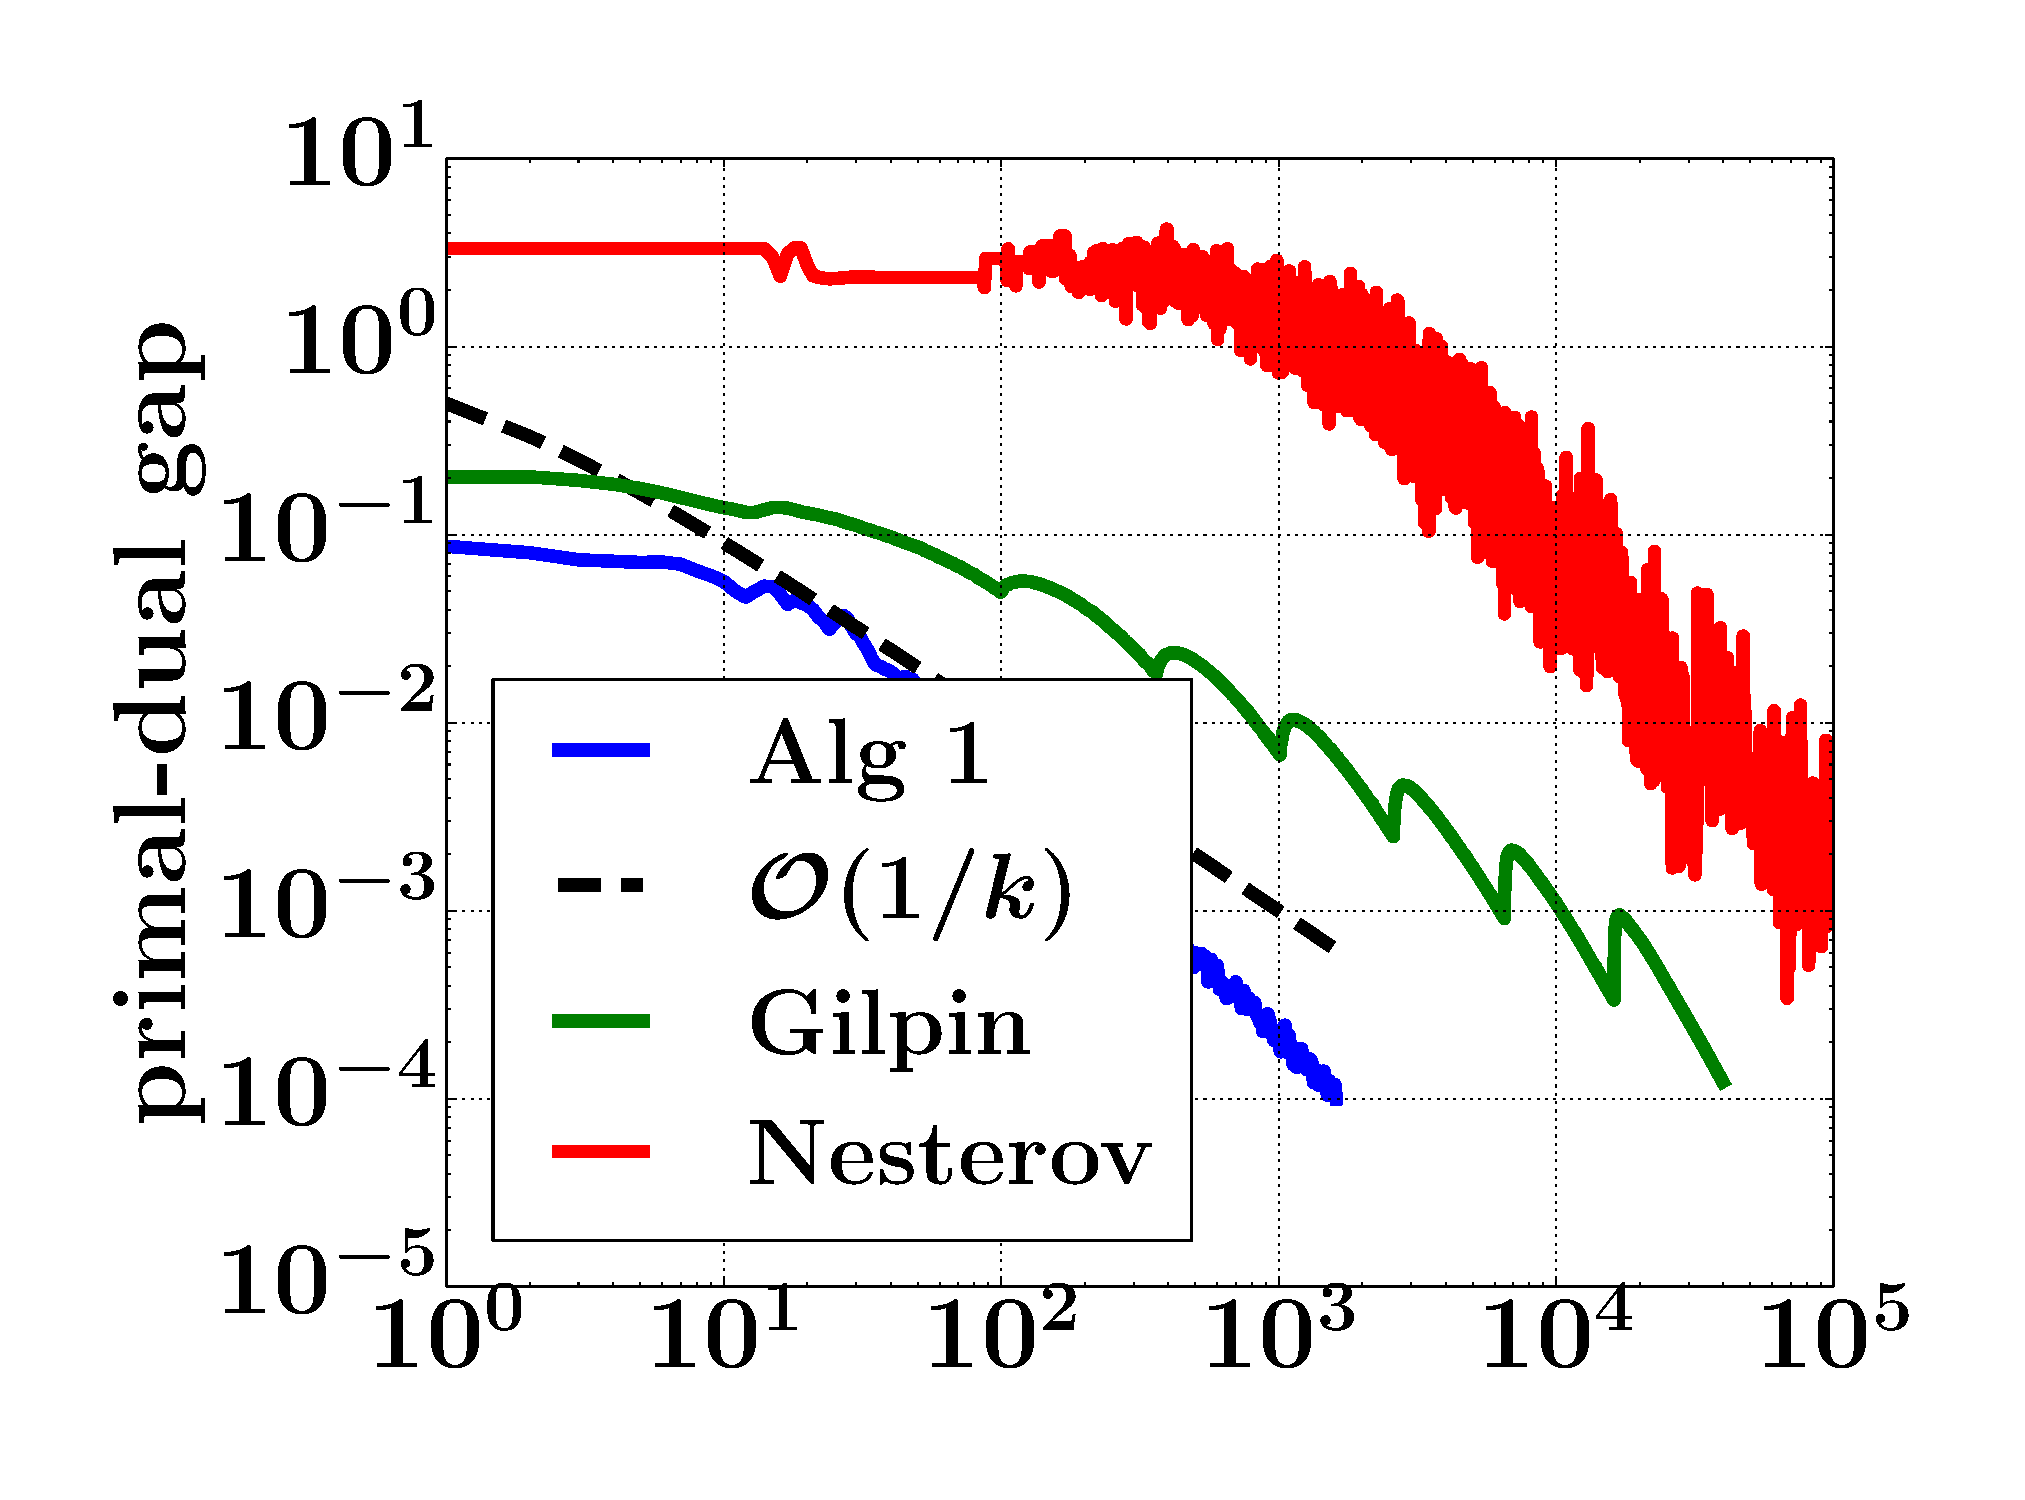
\includegraphics[width=.5\linewidth]{0.pdf}
  }
  %% \hspace{-2em}
  %% \subfigure[Toy Poker]{
  %%   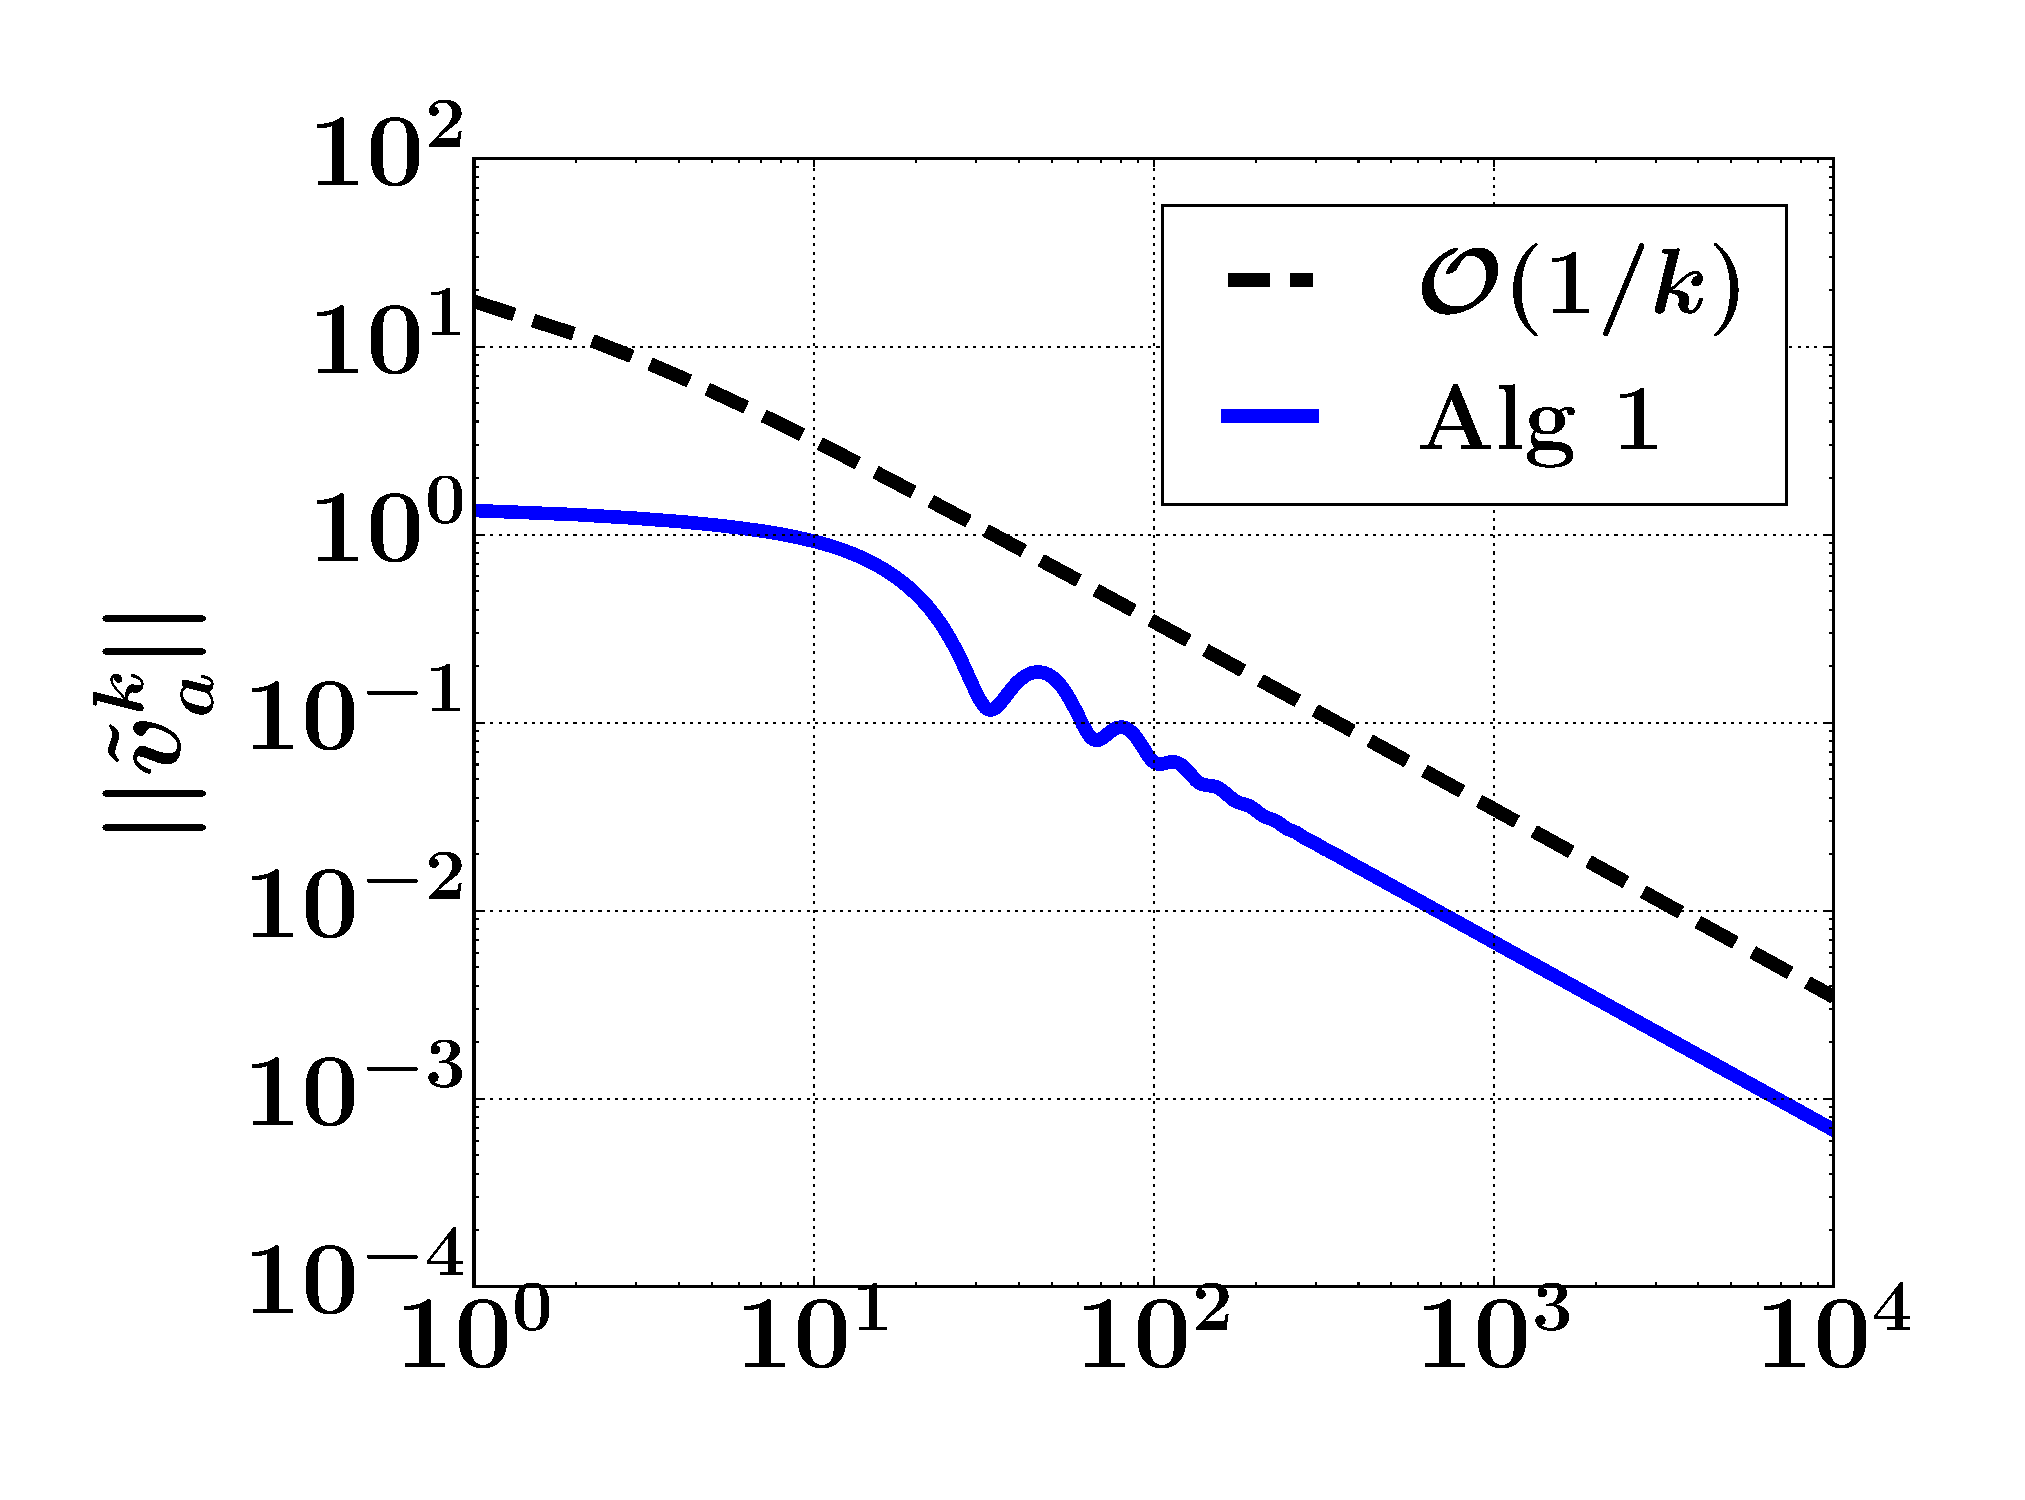
\includegraphics[width=.5\linewidth]{SimplifiedPoker_dgap.pdf}
  %% }
  \hspace{-2em}
  \subfigure[Kuhn 3-card Poker]{
    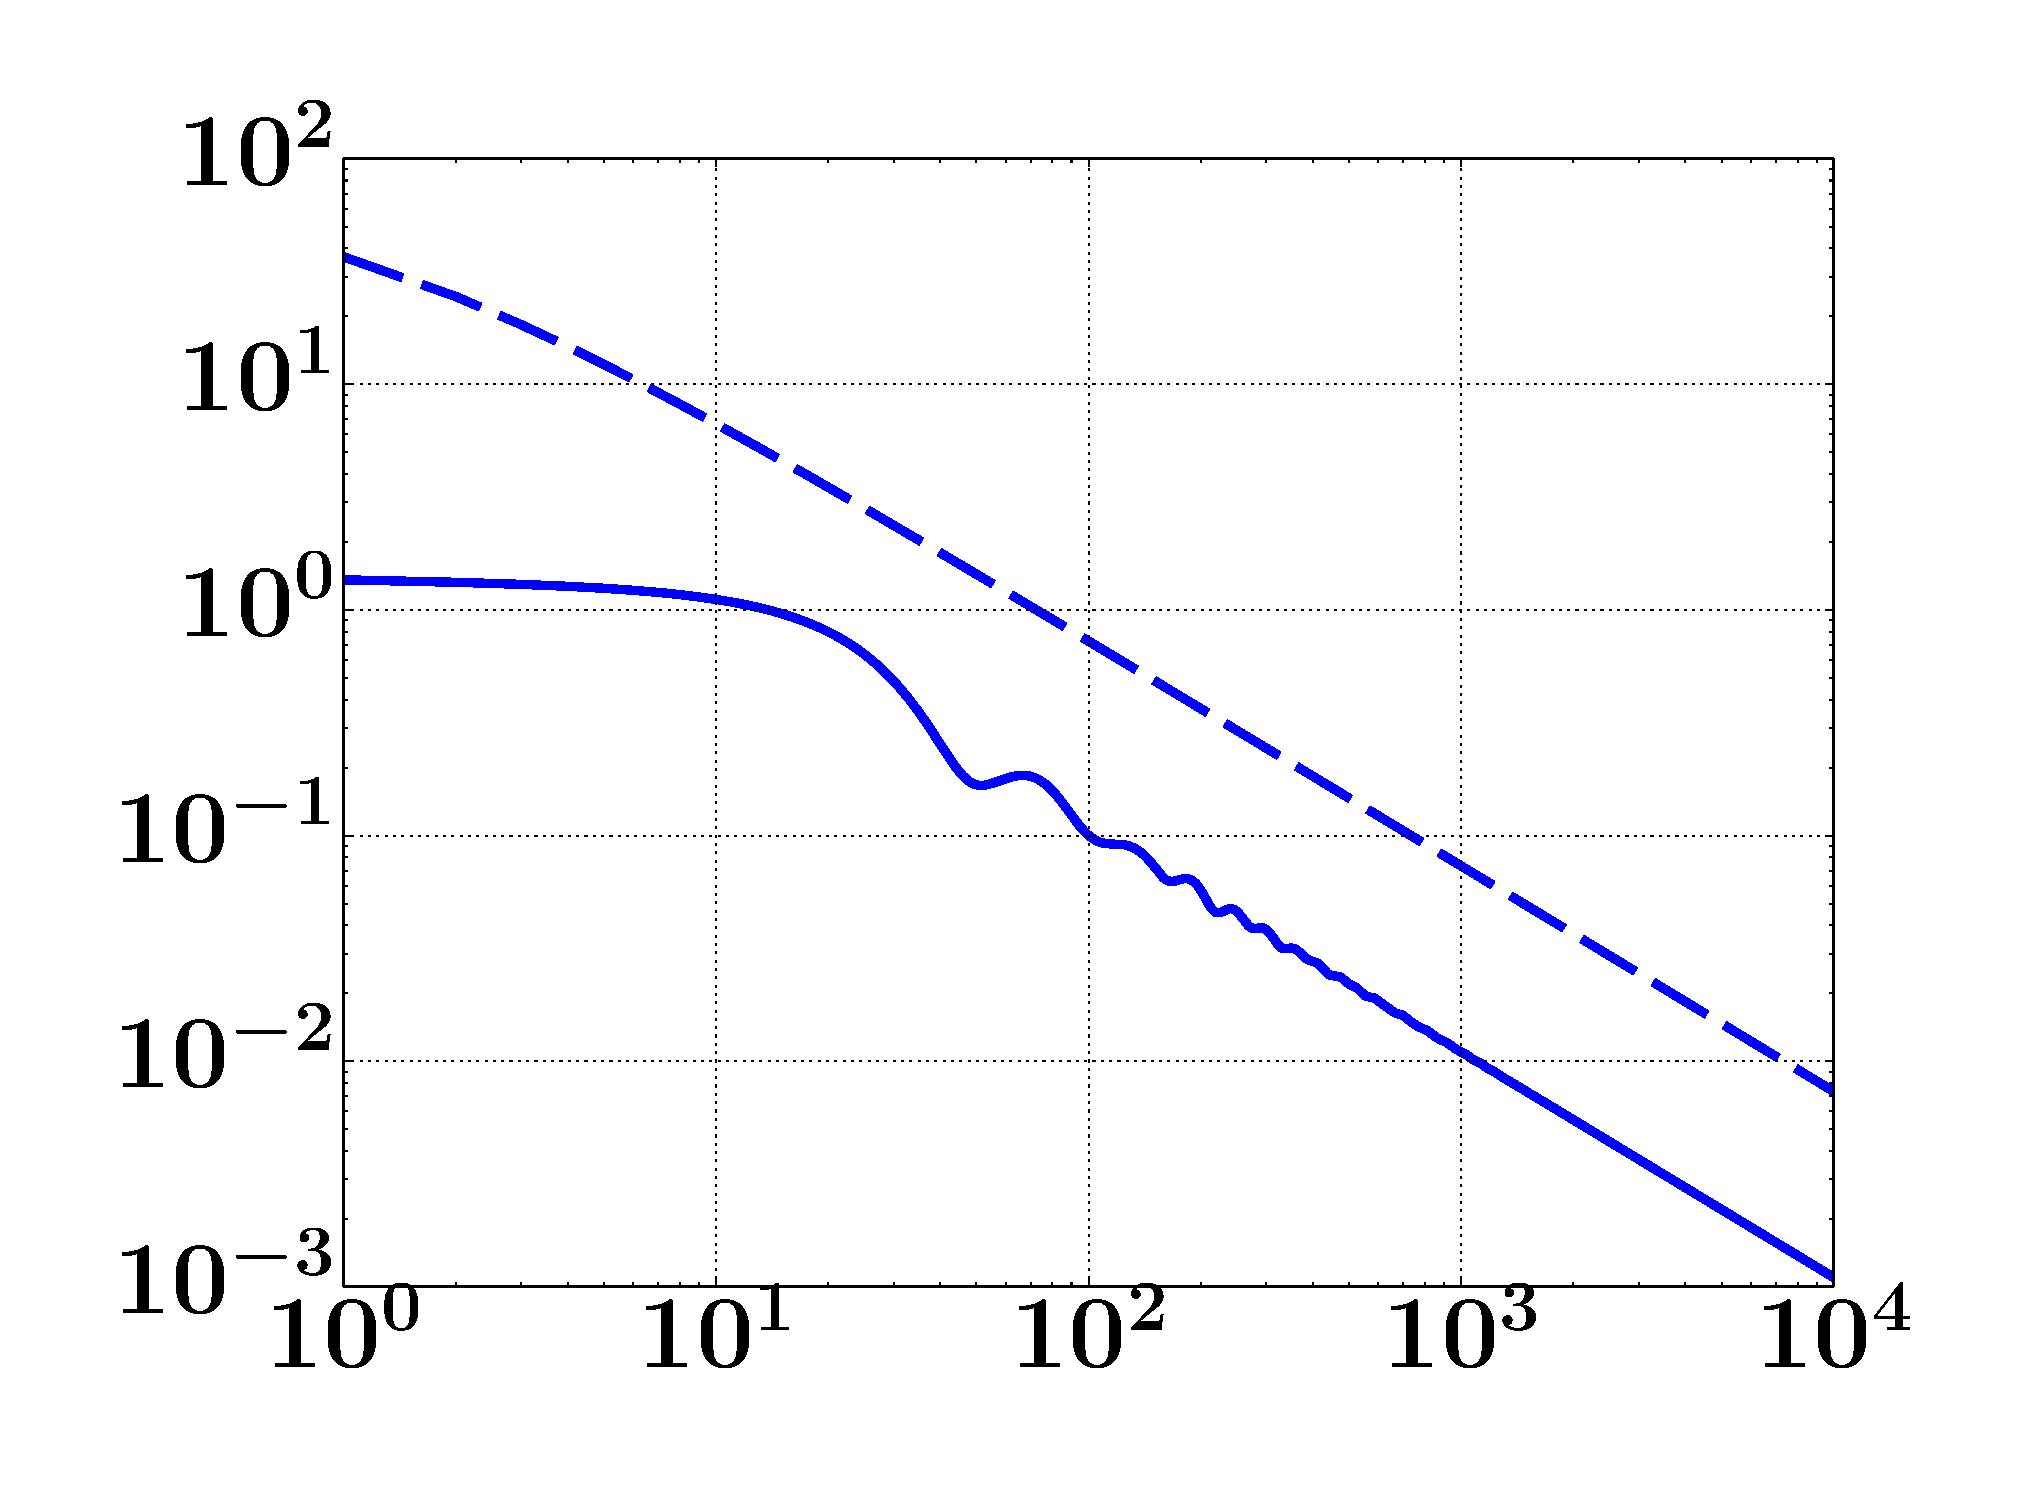
\includegraphics[width=.5\linewidth]{Kuhn3112_dgap.pdf}
  }
  \vspace{-1em}
  \hspace{-2em}
  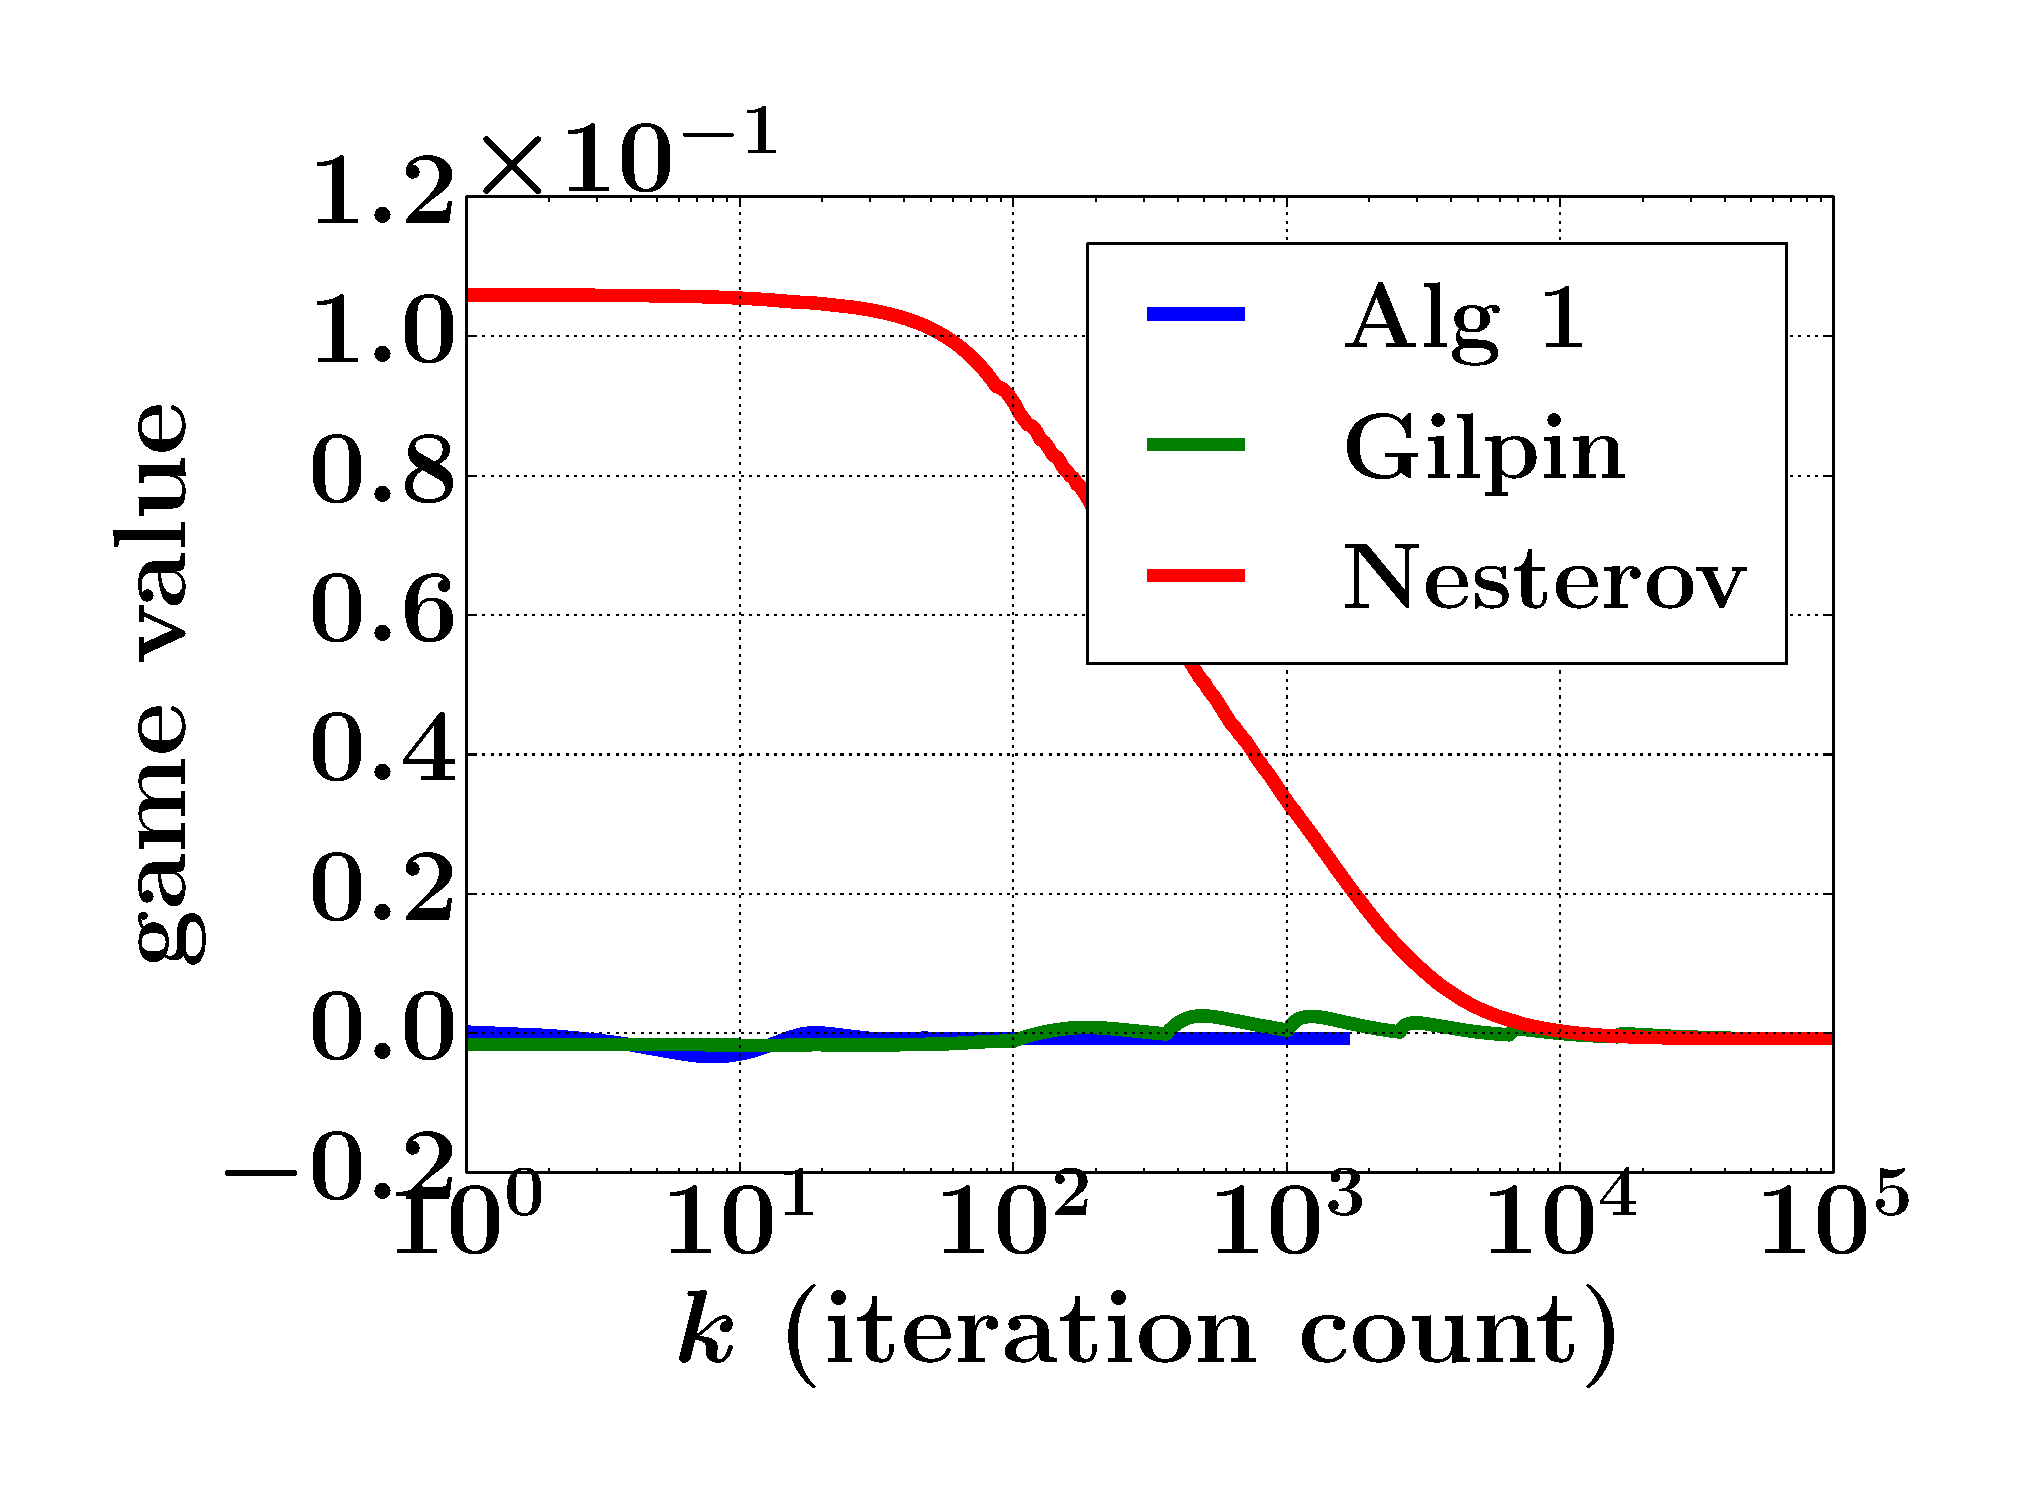
\includegraphics[width=.5\linewidth]{1.pdf}
  %% \hspace{-1em}
  %% 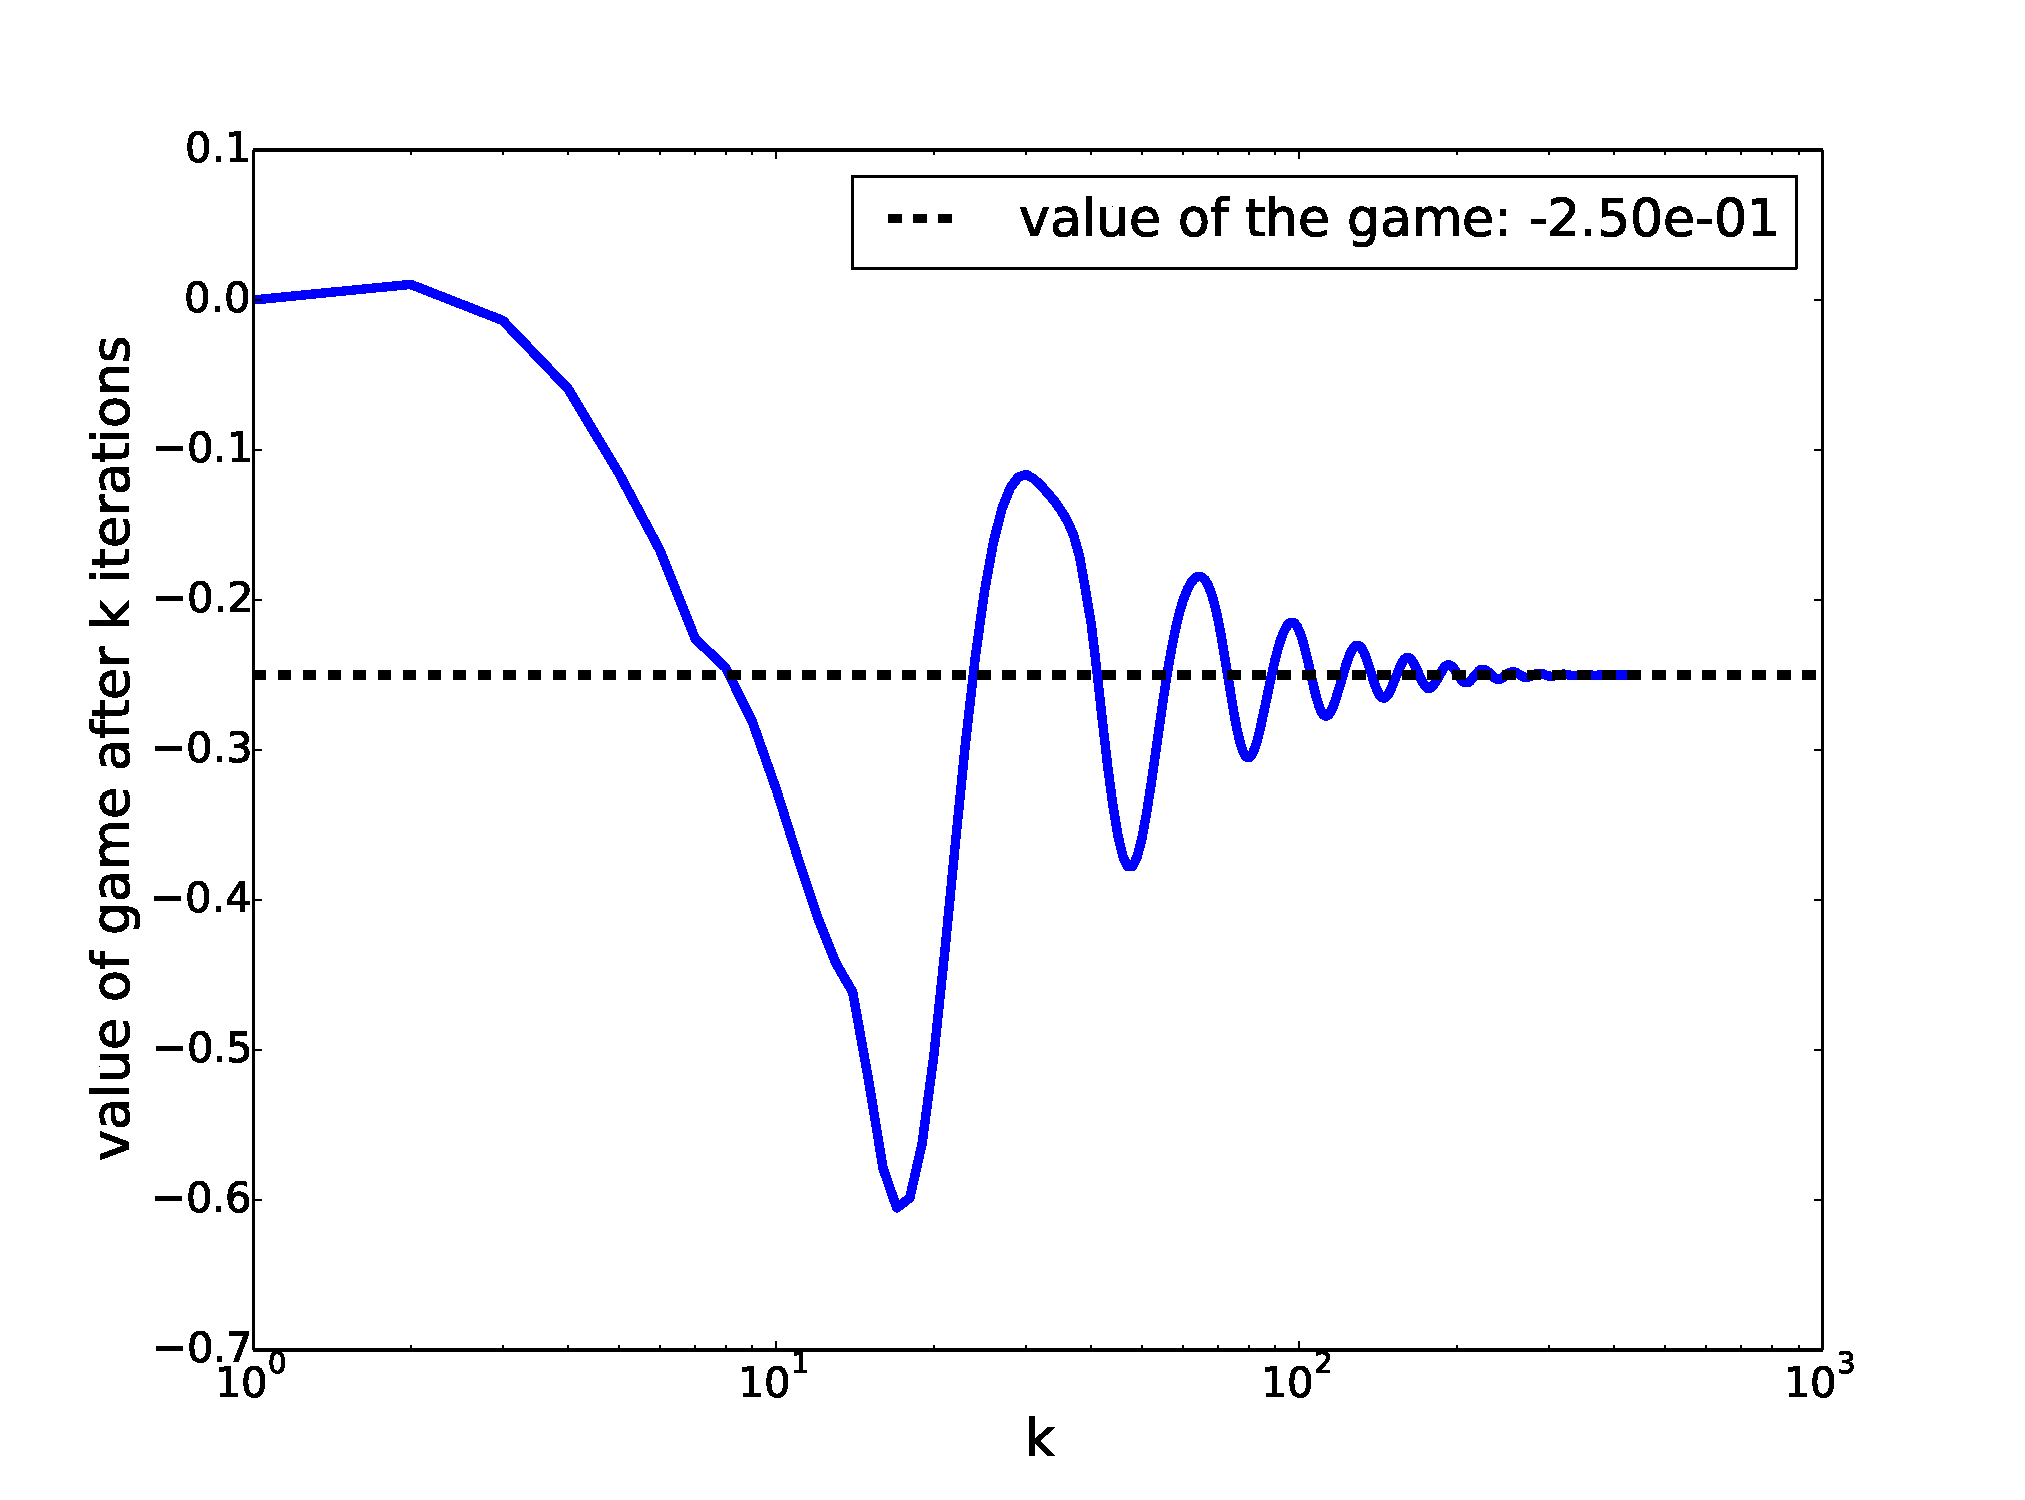
\includegraphics[width=.5\linewidth]{SimplifiedPoker_NE.pdf}
  \hspace{-1em}
  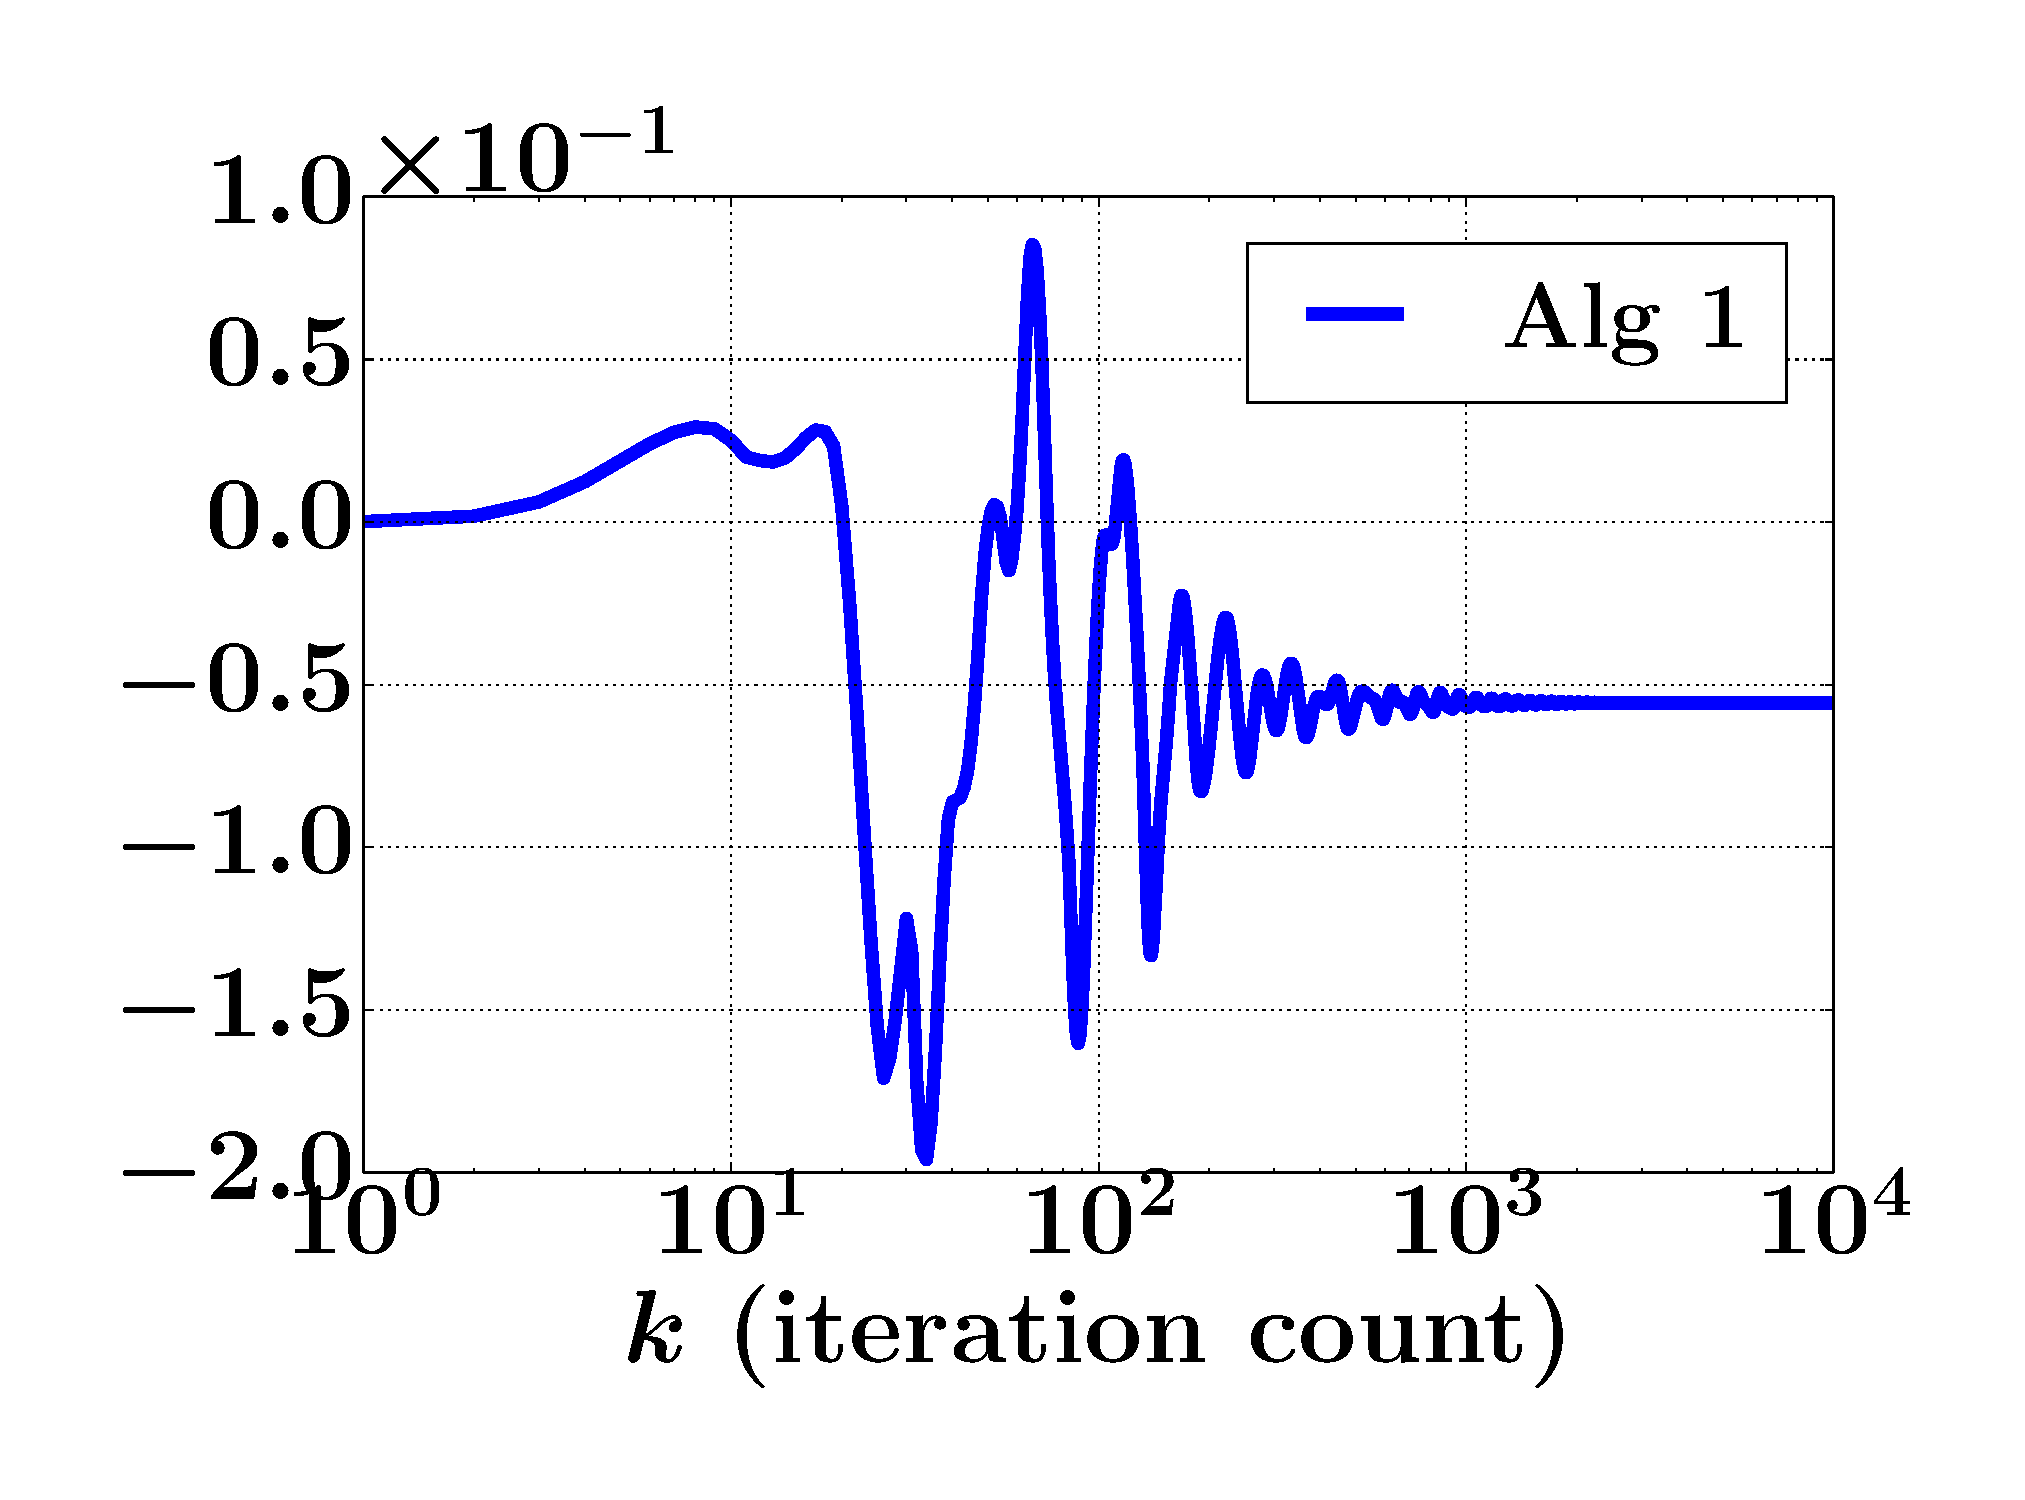
\includegraphics[width=.5\linewidth]{Kuhn3112_NE.pdf}
  \caption{Convergence curves of Algorithm
    \ref{Tab:algo}. \textbf{Top row}: Evolution of ergodic
    primal-dual gap. \textbf{Bottom row}: Evolution of
    value of game.}
  \label{Tab:dgap_curve}
\end{figure}

\paragraph{Experiments on sequential games with imcomplete information: Kuhn 3-card
  poker.} This game is a simplified form of poker
developed by Harold W. Kuhn. It is a two-person zero-sum game which is
simply enough to serve as an example but contains all the complexity
traits of a imcomplete information sequential game. The
deck includes only three playing cards, for example a King, Queen, and
Jack. One card is dealt to each player, then the first player must bet
or pass, then the second player may bet or pass. If any player chooses
to bet the opposing player must bet as well ("call") in order to stay
in the round. After both players pass or bet the player with the
highest card wins the pot. The
sequence-form representation of the game has $n_1 = n_2 = 13$
sequences and $l_1 = l_2 = 7$ information
sets per player. The pair $(x^*, y^*) \in \mathbb{R}^{13} \times
\mathbb{R}^{13}$ of realization plans given by
\begin{eqnarray*}
  \begin{split}
    x^* &= [1, 0.759, 0.759, 0, 0.241, 1, 0.425, 0.575, 0, 0.275, 0,
      0.275, 0.725]^T,\\
    y^* &= [1, 1, 0, 0.667, 0.333, 0.667, 0.333, 1, 0, 0, 1, 0, 1]^T
    \end{split}
\end{eqnarray*}
is a Nash $10^{-4}$-equlibrium computed in 1500 iterations of
Algorithm  \ref{Tab:algo}. The convergence curves are shown
in Fig \ref{Tab:dgap_curve}. One easy checks that this equilibrium is
feasible. Indeed, $E_1x^* - e_1 = [4.76 \times 10^{-5}, -1.91 \times 10^{-5}, 5.67
      \times 10^{-5}, 8.23 \times 10^{-6}, 2.90 \times 10^{-5},
      -8.62 \times 10^{-7}, -1.96 \times 10^{-5}]^T$
and
$E_2y^* - e_2 = [-7.04 \times 10^{-7}, 2.27 \times 10^{-6}, -3.29
  \times 10^{-6}, -1.50 \times 10^{-6},
      2.92 \times 10^{-6}, -4.97 \times 10^{-7}, -5.85 \times
      10^{-7}]^T$.
Finally, one checks that ${x^*}^TAy^* = {-0.05555}$,
 which agrees to 5 d.p with the value of $-1 / 18$ computed
 analytically by H. W. Kuhn in his 1950 paper \cite{kuhn}. The
 evolution of the dual gap and the expected value of the game across
 iterations are shown in Figure \ref{Tab:dgap_curve}.
More details (payoff matrix, etc.) are provided in
the supplementary materials...

\section{Concluding remarks}
Making use of the sequence-form representation
\cite{koller1992complexity,von1996efficient,vonequilibrium}, we have
deviced a simple and efficient primal-dual algorithm for computing
Nash equilibria in two-person zero-sum sequential games with
imcomplete information (like Texas Hold'em, etc.). Our algorithm is
simple to implement, with a very low constant cost per iteration, and
enjoys a rigorous convergence theory with a proven
$\mathcal{O}(1/\epsilon)$ convergence in terms of basic operations
(matvec products, clipping, etc.), to a Nash
$(\epsilon,0)$-equilibrium of the game. Equilibrium problems are
saddle-point convex-concave problems, and as
such a natural choice for algorithms for solving them would be in the
family of primal-dual algorithms. We believe such primal-dual
schemes will receive more attention in the algorithmic game theory
community in future.

The author's implementation of the proposed algorithm is available
upon request.

%% \paragraph{About the author:} I'm a first-year PhD student in Computer
%% Science at Universit\'e de Parix XI. My thesis focuses on novel
%% techniques for optimization on Lie groups (of diffeomorphisms), and
%% other structured manifolds, the aim being to obtain better algorithms
%% for nonlinear registration of fMRI brain images and enhance the
%% charting of human functional connectomes.
%\pagebreak
\bibliographystyle{llcns2e/splncs03}
\bibliography{bib}


\section{Supplementary materials}
\subsection{Sequence-form representation for Kuhn 3-card poker}
$E_1 \in \mathbb{R}^{7 \times 13}$ with $E_1(0,0) = E_1(1,9) =
E_1(1,12) = E_1(2,1) = E_1(2,4) = E_1(3,5) =
E_1(3,8) = E_1(4,2) = E_1(4,3) = E_1(5,6) = E_1(5,7) = E_1(6,10) =
E_1(6,11) = {1}$, $E_1(1,0) = E_1(2,0) = E_1(3,0) = E_1(4,1) =
E_1(5,5) = E_1(6,9) = {-1}$; \\

 $E_2 \in \mathbb{R}^{7 \times 13}$ with
$E_2(0,0) = E_2(1,7) = E_2(1,8) = E_2(2,9) = E_2(2,10) = E_2(3,5) =
E_2(3,6) = E_2(4,11) = E_2(4,12) = E_2(5,1) = E_2(5,2) = E_2(6,3) =
E_2(6,4) = {1}$, $E_2(1,0) = E_2(2,0) = E_2(3,0) = E_2(4,0) =
E_2(5,0) = E_2(6,0) = {-1}$; and \\

 $A \in \mathbb{R}^{13 \times
  13}$ with $A(3,8) = A(3,12) = A(4,6) = A(4,10) = A(7,12) = A(8,10) =
{-0.333333}$, $A(1,7) = A(1,11) = A(2,8) = A(2,12) = A(5,11) =
A(6,4) = A(6,12) = A(10,4) = A(10,8) = {-0.166667}$, $A(7,4) =
A(8,2) = A(11,4) = A(11,8) = A(12,2) = A(12,6) = {0.333333}$,
$A(4,5) = A(4,9) = A(5,3) = A(8,1) = A(8,9) = A(9,3) = A(9,7) =
A(12,1) = A(12,5) = {0.166667}$.\\


%\paragraph{\textbf{Toy Poker game...}}
%% The sequence-form representation for this Toy Poker game is given by
%% (showing only nonzero entries):\\

%% $E_1 \in \mathbb{R}^{3 \times 5}$ with $E_1(0,0) = E_1(1,1) =
%% E_1(1,2) = E_1(2,3) = E_1(2,4) = {1}$,
%% $E_1(1,0) = E_1(2,0) = {-1}$; \\

%% $E_2 \in \mathbb{R}^{3 \times 5}$ with $E_2(0,0) = E_2(1,1) = E_2(1,2)
%% = E_2(2,3) = E_2(2,4) = {1}$, $E_2(1,0) = E_2(2,0) =
%% {-1}$; and \\

%% $A \in \mathbb{R}^{5 \times 5}$ with $A(2,0) =
%% A(4,0) = {-0.5}$, $A(1,3) = {1}$, $A(3,1) =
%% {-1}$, $A(1,2) = A(1,4) = A(3,2) = A(3,4) = {0.25}$.



\end{document}
